% *//   MODELE DE DOCUMENT LaTeX //* 
% -----------------------------------
% Inclut sections, sous-sections et sous-sous-sections.
% Examples d'intégration de figures, de tableaux et d'algorithme.
% -----------------------------------
% Gestion automatique de la mise en forme biblio grâce à BibTeX.
% Il suffit de copier le code BibTeX de la publication dans le fichier 'biblio.bib'.
% Sur GScholar : cliquer sur Citer puis BibTeX.
% Citer ensuite le papier comme dans l'example de l'introduction. 
% La bibliographie sera automatiquement mise en forme à la fin du document aux normes APA. 
% -----------------------------------
\documentclass[12pt,a4paper]{report}
\usepackage[utf8]{inputenc}
\usepackage{graphicx,setspace,csquotes}
\usepackage[T1]{fontenc}
\usepackage[skip=12pt, indent=30pt]{parskip}
\usepackage[english,french]{babel}
\usepackage[autolanguage]{numprint}
\usepackage[backend=biber,style=numeric,sorting=none]{biblatex}
\usepackage[font=small,labelfont=bf]{caption}
\usepackage{geometry}
% \usepackage[a4, a3, landscape]{geometry}
\usepackage{booktabs}
\usepackage[french]{algorithm2e}
\usepackage{float}
\usepackage{hyperref}
\def\frenchtablename{Tableau}
\usepackage{caption}
\usepackage{subcaption}
\usepackage[dvipsnames, table]{xcolor}
\usepackage{array}
\usepackage{lmodern}
\usepackage{enumitem}
\usepackage{tabularx} 
\usepackage{booktabs} 
\usepackage{blindtext}
\usepackage{longtable}
\usepackage{booktabs}
\usepackage{amsmath}
\usepackage{titlesec} 
\usepackage{tocloft}
\usepackage{etoolbox}
\usepackage{titletoc}   
\usepackage[Lenny]{fncychap}
\usepackage{etoc}
\usepackage{fancyhdr}
\usepackage{afterpage}
\usepackage{arabtex}
\usepackage{pdfpages}
\usepackage[export]{adjustbox}
\setcode{utf8}
\setcounter{secnumdepth}{3}
\titleformat*{\section}{\LARGE\bfseries}
\titleformat*{\subsection}{\Large\bfseries}
\titleformat*{\subsubsection}{\large\bfseries}
\titleformat*{\paragraph}{\large\bfseries}
\titleformat*{\subparagraph}{\large\bfseries}
%\usepackage{enumitem}
% \titleformat{\chapter}[display]
%   {\normalfont\bfseries\Huge}
%   {\filleft\Large\chaptertitlename\ \thechapter}
%   {4ex}
%   {\titlerule\vspace{2ex}\filright}
%   [\vspace{2ex}\titlerule]

\pagestyle{fancy}
\fancyhf{}  % Clear all header and footer fields
\fancyhead[L]{\hspace{10pt}\leftmark}
\fancyfoot[C]{\thepage}  % Center footer

\addbibresource{biblio.bib}

% Configuration des liens
\definecolor{personalizedColor}{RGB}{0, 163, 166}
\hypersetup{
    colorlinks=true,
    linkcolor=black,
    filecolor=black,      
    urlcolor=personalizedColor,
    citecolor=personalizedColor,
    pdftitle={Rapport Final},
    pdfpagemode=FullScreen,
    }
\urlstyle{same}
% Configuration des algorithmes
\RestyleAlgo{ruled}
\SetKw{KwBy}{by}
% Configuration des légendes
\captionsetup{width=13.5cm}

% \geometry{margin=0.5in}
\geometry{
  paperwidth=210mm, 
  paperheight=297mm,
  margin=0.5in,
  top=1in,
  headheight=15pt  
}

\fancypagestyle{empty}{
  \fancyhf{}  % clear all header and footer fields
  \renewcommand{\headrulewidth}{0pt}  % no line in header area
}

\begin{document}

\newgeometry{margin=0.5in}
\begin{titlepage}
    \begin{center}
        
\includegraphics[width=.50\textwidth]{logos/isgs.png}
    
        \vspace*{0.5cm}
        \large
        \textbf{Ministère de l'Enseignement Supérieur et de la Recherche Scientifique}
        
        \vspace*{0.3cm}
        \textbf{***}

        \vspace*{0.3cm}
        \textbf{Université de Sousse}

        \vspace*{0.3cm}
        \textbf{***}

        \vspace{0.3cm}
        \textbf{Institut Supérieur de Gestion de Sousse}

        \vspace{0.3cm}
        \large
        \vspace*{0.3cm}
        \textbf{License en Informatique de Gestion (Business Intelligence)}\\

        \vspace*{0.3cm}
        \textbf{Rapport de Stage de Fin D'Études}

        \large
        \vspace*{0.3cm}
        \textbf{Amelioration de recherche et intégration de Recherche Intelligent}\\
            
        \vspace{1cm}
        \large
        \textbf{Borgi Aaron et Ben Hassine Ghaithallah}\\
        3éme LIG\\
        \vspace{0.5cm}
        
        \textbf{Encadreur de stage: } Haddad Ahmed \\        
        \textbf{Référent universitaire: } Haddad Ahmed \\
        \textbf{Année Universitaire: } 2023-2024
        
    \end{center}
\end{titlepage}
\restoregeometry

\spacing{1.5}

\pagenumbering{gobble}
\thispagestyle{empty}
\begin{center}
	\LARGE\textbf{Remerciements}
\end{center}
\vspace{0.5cm}
\large
\noindent
Nous voudrons remercier tous ceux qui ont participé à mener ce projet. Nous tenons spécialement à remercier: \\

\noindent
Monsieur, Ahmed Haddad, pour son encadrement, son soutien, ses conseils qui nous ont été d'une grande utilité pour rédiger, pour l'aide et le support tout au long de ce project, ses conseils ont été d'un grand apport.

\vspace{0.5cm}
\noindent
Nos remerciements vont aussi à tous les professeurs de l'ISGS, pour leurs générosités et la patience dont ils ont su faire preuve.

\newpage

\pagenumbering{gobble}
\thispagestyle{empty}
\begin{center}
\LARGE\textbf{Dédicace}
\end{center}

\large
\noindent
A nos parents, qui nous ont aidé à devenir ce que nous sommes aujourd’hui,\par
\vspace{12pt}
\noindent
A nos amis et à nos proches,\par
\vspace{12pt}
\noindent
A tous ceux qui nous ont aidé à accomplir ce projet…\par
\vspace{12pt}
\noindent
Toute notre reconnaissance.

\newpage


\tableofcontents
\listoffigures
\listoftables
\newpage

\chapter{Sprint 0: Planification du projet}
\etocsettocstyle{\section*{Sommaire}}{}
\localtableofcontents
\section{Introduction}
\noindent
Dans ce chapitre, on va présenter la premiére phase de la méthode SCRUM, qui est le Sprint 0, qui commence par l'identification des besoins. Par la suite, nous faisons une analyse globale de notre projet en identifiant les acteurs et ensuite le diagramme de cas d'utilisation globale. De plus, nous planifions le reste des sprints de notre projet. Puis, on va présnter l'architecture du systéme pour laquelle nous avons opté. Et enfin, on va présenter les outils de développement utilisés pour réaliser ce projet.

\section{Identification des besoins}
\subsection{Les besoins fonctionnels}
\noindent
Les besoins fonctionnels sont les fonctionnalités que le systéme doit livrer aux utilisateurs.
L’outil n’est considéré comme opérationnel que si sa disponibilité fonctionnelle est garantie.
Dans le cas du notre systéme, ces besoins se concentrent sur:

\begin{itemize}
    \item \small\textbf{Vitesse de recherche: } {Améliorer les vitesses de recherche au maximum afin de renvoyer des résultats précis au client.}
    
    \item \small\textbf{Recherche en Français: } {Permettre le client a rechercher les produits dans la langage Française.}

    \item \small\textbf{Recherche en Arabe Tunisienne: } {Permettre le client a rechercher les produits dans la langage Arabe Tunisienne.}

    \item \small\textbf{Recherche en Arabe Traditionnel: } {Permettre le client a rechercher les produits dans la langage Arabe Classique.}
    
    \item \small\textbf{Suggestion des produits: } {Si le produit recherché par le client n'existe pas, le système tentera de suggérer des produits similaires en prenant le contexte du terme de recherche.}
\end{itemize}

\newpage
\subsection{Les besoins non fonctionnels}
\noindent
Les exigences non fonctionnels décrivent les objectifs liés aux performances du systéme et d'autres aspects cruciaux du système qui ne sont pas directement liés à ses fonctionnalités spécifiques. Ils définissent les critères de qualité que le système doit respecter pour répondre aux attentes des utilisateurs. Notre systéme doit repondre aux exigences non fonctionnels suivantes:

\begin{itemize}
    \item \small\textbf{La Fiabilité: } L'application doit être fonctionnelle sans détection des erreurs afin de satisfaire les besoins de client.

    \item \small\textbf{La Sécurité: } Vu que l'application contient des données confidentielles, tous l'accés des produits doivent être protégées par un privilege d'accées.

     \item \small\textbf{La Disponibilité: } Les services offerts par notre application sont disponibles pendant les 24
     heures et durant toute la semaine.

     \item \small\textbf{La Performance: } L'application doit être rapide et robuste (Vitesse de réponse rapide et précision des résultats lors du recherche des produits dans les langues différents).
\end{itemize}

\newpage
\section{Diagramme de cas d’utilisation global}
\subsection{Introduction}
\noindent
Dans cette partie, on va présenter les besoins de notre systéme de façon formelle à l'aide du diagramme de cas d'utilisation du langage de modélisation UML. D'abord nous identifions les acteurs qui intéragissent avec notre systéme, qui sont:

\noindent
\small\textbf{Le Visiteur: } C'est le personne qui va accéder à notre systéme pour rechercher le(s) produit(s) dans notre systéme.

\noindent
\small\textbf{Le Client: } C'est aussi le personne qui va accéder à notre systéme pour rechercher le(s) produit(s) de ses besoins. 

\noindent
\small\textbf{L'Admin: } C'est le personne qui va accéder à notre systéme pour rechercher le(s) produit(s) dans notre systéme et modifier les paramétres de son recherche. 

\begin{figure}[H]
\centering
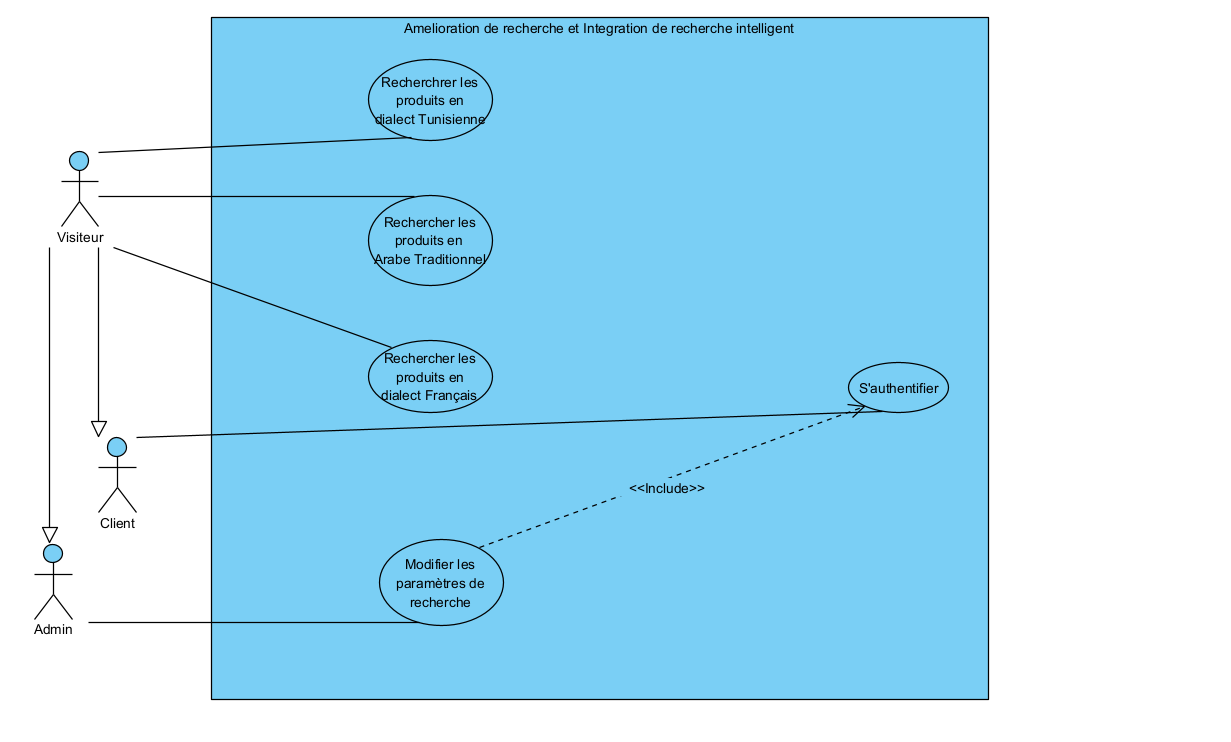
\includegraphics[width=1\textwidth]{logos/CU_global.png}
\caption{Présentation de Diagramme de Cas D'Utilisation global}
\label{fig:diagcuglobal}
\end{figure}
\section{Backlog De Produit}
\noindent
\large
Le backlog de produit est une liste de fonctionnalités à réaliser. Ces fonctionalités sont exprimées sous formes des besoins et sont priorisées par le Product Owner ce qui permet d'établir un ordre de réalisation à respecter. \\
Notre backlog est composé de trois colonnes: \\
\textbf{ID: } C'est l'identifiant du scénario \\
\textbf{Fonctionnalité: } Permet de mieux ordonner les scénarios. \\
\textbf{Scénario: } Comporte la description des scénarios suivant le forme << En tant que ... Je veux >> \\

\begin{table}[H]
\centering
\begin{tabular}{|c|c|p{10cm}|}
\hline
\rowcolor{blue!20}
\textbf{ID} & \textbf{Fonctionnalité} & \textbf{Scénario} \\ \hline
1 & Recherche en Arabe Tunisienne  & En tant qu'un client, je veux rechercher un ou plusieurs produits dans la langue Tunisienne. \\ \hline
2 & Recherche en Arabe Classique & En tant qu'un client, je veux rechercher un ou plusieurs produits en Arabe Classique. \\ \hline
3 & Recherche en Français & En tant qu'un client, je veux rechercher un ou plusieurs produits en Français. \\ \hline
4 & Vitesse de recherche & En tant qu'un client, je veux avoir une vitesse de recherche rapide. \\ \hline
5 & Suggestion des produits & En tant qu'un client, si le produit que je cherche n'existe pas, je veux avoir des suggestions des produits similaires. \\ \hline
\end{tabular}
\caption{Table des fonctionnalités et scénarios.}
\end{table}
\section{La Plannification De Release}
\noindent
Une fois que le Product Owner a fini de construire le Product Backlog, l'équipe SCRUM et l'environnement technique du projet est bien mis en œuvre, et tous le membres du projet sont plannifiés le sprint ensemble aussi que les fonctionnalités à développer pour chaque Sprint, la durée de la prévision de chaque sprint est estimée à quatre semaines.
\section{Architecture du systéme}
\noindent
Il est indispensable à la conception de tout systéme informatique de choisir le modéle d'architecture adéquat et pourra assurer le bon fonctionnement, une meilleure performance, ainsi que la scalabilité, la fiabilité et trés important, la productivité de développement. \\
C'est pour cette raison, qu'on a opté pour l'architecture MVC avec des microservices (Modèle, Vue, Contrôleur, Modèle IA, et Elasticsearch) comme l'architecture global du projet, et le modèle << Clean Architecture >>, dans le backend, qui seront trés pratique pour gérer les intéractions entre les différents composants de notre application. Nous décrirons ces architectures dans les prochaines sections.

\subsection{Architecture "MVC Avec Microservices"}
\noindent
Le modèle MVC permet de bien organiser son code source. Il va nous aider à savoir quels fichiers créer, mais surtout à définir leur rôle. Le but de MVC est justement de séparer la logique du code en trois parties que l'on retrouve dans des fichiers distincts.

\noindent
{\small\textbf{\textit{Modèle}}}\mbox{}\\
Cette partie gère ce qu'on appelle la logique métier de notre site. Elle comprend notamment la gestion des données qui sont stockées, mais aussi tout le code qui prend des décisions autour de ces données. Son objectif est de fournir une interface d'action la plus simple possible au contrôleur. On y trouve donc entre autres des algorithmes complexes et des requêtes SQL, et Elasticsearch dans notre cas.

\noindent
{\small\textbf{\textit{Vue}}}\mbox{}\\
Cette partie se concentre sur l'affichage. Elle ne fait presque aucun calcul et se contente de récupérer des variables pour savoir ce qu'elle doit afficher. On y trouve essentiellement du code HTML mais aussi quelques boucles et conditions Javascript très simples, pour afficher par exemple une liste de messages. Il est développé avec React et Typescript.

\noindent
{\small\textbf{\textit{Contrôleur}}}\mbox{}\\
Cette partie gère les échanges avec l'utilisateur. C'est en quelque sorte l'intermédiaire entre l'utilisateur, le modèle et la vue. Le contrôleur va recevoir des requêtes de l'utilisateur. Pour chacune, il va demander au modèle d'effectuer certaines actions (demander les produits en fonction d'un mot-clé de recherche) et de lui renvoyer les résultats (la liste des produits). Puis il va adapter ce résultat et le donner à la vue. Enfin, il va renvoyer la nouvelle page HTML, générée par la vue, à l'utilisateur. Il est implémenté avec ASP .NET Core et C\# et utilise des requêtes SQL et Elasticsearch pour manipuler les donnèes.

\noindent
{\small\textbf{\textit{Modèle IA}}}\mbox{}\\
Notre modèle IA a une et une seule responsabilité, qui est de faire l'encodage de la requête de l'utilisateur qui est envoyé au contrôleur et retourner le résultat encodé.

\noindent
{\small\textbf{\textit{Elasticseach}}}\mbox{}\\
Elasticsearch agit comme notre base de données de recherche de vecteurs qui contient notre index de produits contenant 2 colonnes de vecteurs recherchables à l'aide du vecteur codé renvoyé par le modèle AI.

\newpage
\noindent
La figure ~\ref{fig:mvc} schématise le rôle de chacun de ces éléments.
\begin{figure}[H]
\centering
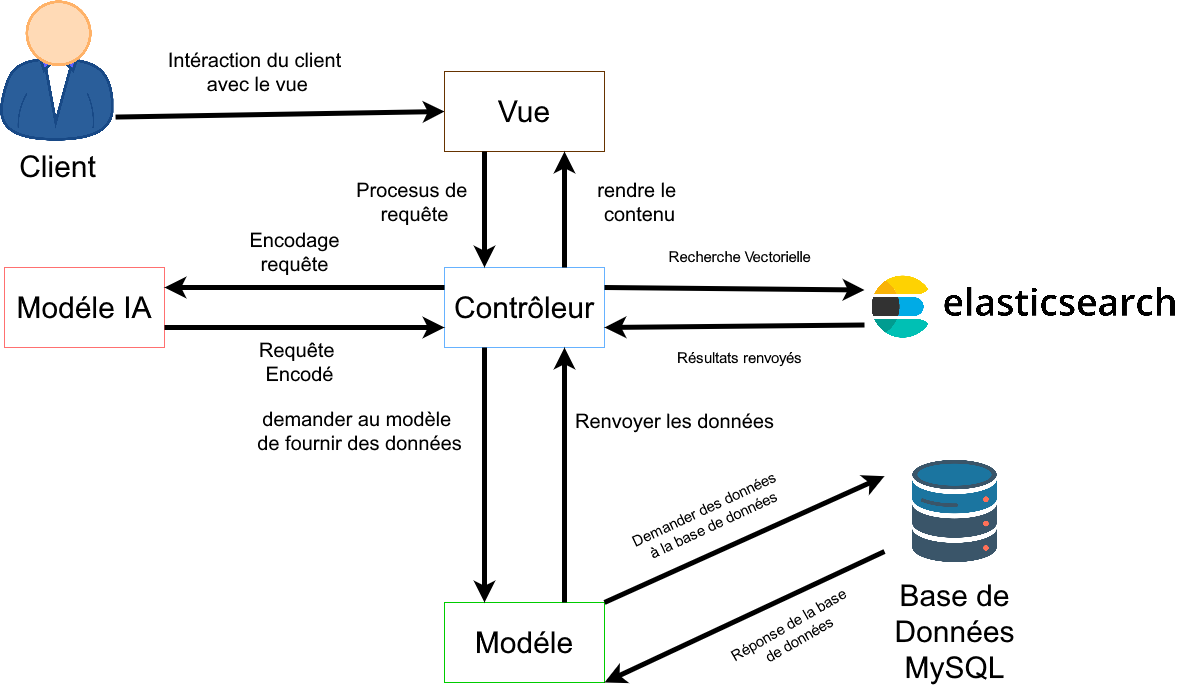
\includegraphics[width=1\textwidth]{logos/mvcavecservice.png}
\caption{L'architecture MVC avec microservices}
\label{fig:mvc}
\end{figure}

\noindent
Il est important de bien comprendre comment ces éléments s'agencent et communiquent entre eux. La figure ~\ref{fig:mvcechange} montre cette communication.

\begin{figure}[H]
\centering
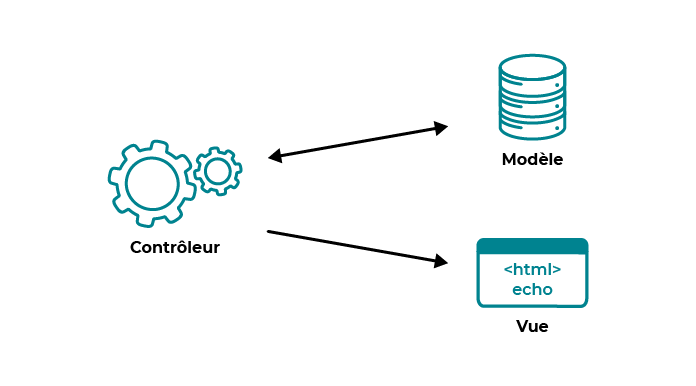
\includegraphics[width=1\textwidth]{logos/mvcechange.png}
\caption{Échange d'informations entre les éléments MVC}
\label{fig:mvcechange}
\end{figure}

\subsection{Architecture "Clean Architecture"}
\noindent
"Clean Architecture" est un modèle architectural introduit par Robert C. Martin, également connu sous le nom d'Oncle Bob. Il favorise une séparation claire des préoccupations en divisant l'application en couches concentriques, chaque couche ayant ses responsabilités et ses dépendances. Le principe fondamental derrière l'architecture propre est la règle de dépendance, qui stipule que les dépendances doivent toujours pointer vers l'intérieur vers les couches les plus stables et abstraites, plutôt que vers l'extérieur vers des couches plus concrètes et volatiles. 

\noindent
Cette architecture se compose généralement des couches suivantes: \\

\begin{itemize}
    \small\item \textbf{La couche Presentation: } Cette couche est responsable de la gestion des interactions des utilisateurs et de la fourniture des données à l'interface utilisateur. Dans notre context d'une API Web .NET Core, cette couche comprend les contrôleurs et autres composants qui gèrent les requêtes et les réponses HTTP.

    \small\item \textbf{La couche Application: } La couche Application contient la logique métier et les cas d’utilisation de l’application. Il agit comme intermédiaire entre la couche présentation et la couche domaine. Cette couche est indépendante de tout problème spécifique d’interface utilisateur ou d’infrastructure.
    \small\item \textbf{La couche Domain: } La couche Domain représente le noyau de l’application, encapsulant les règles métier, les entités, les interfaces (Orienté Objet) des repositories des bases de donnés et la logique spécifique au domaine. Il doit être indépendant de la technologie et ne contenir aucune dépendance vis-à-vis de frameworks ou de bibliothèques externes.

    \small\item \textbf{La couche Infrastructure: } La couche infrastructure traite des problèmes externes tels que les bases de données, les services externes et les frameworks. Il contient des implémentations d'interfaces définies dans la couche application et interagit avec des ressources externes.
\end{itemize}

\noindent
La figure Figure~\ref{fig:architecture} reprèsente les couches de << Clean Architecture >>

\begin{figure}[H]
\centering
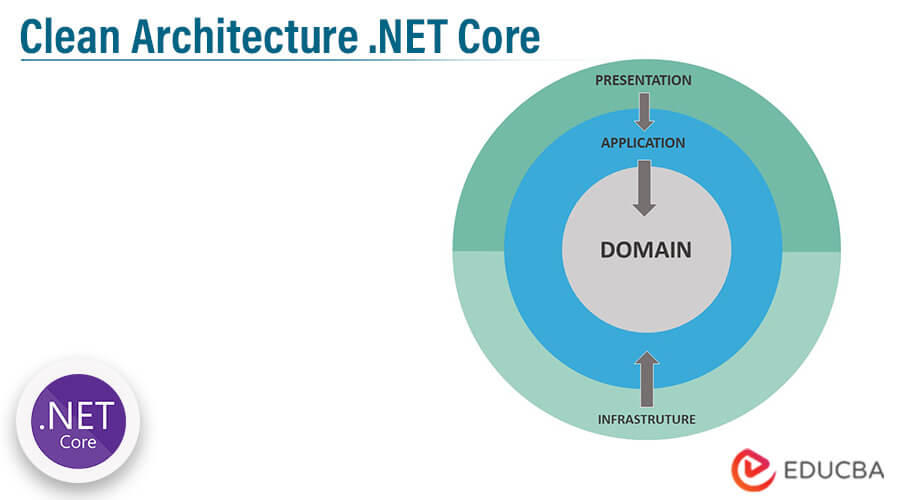
\includegraphics[width=1\textwidth]{logos/clean_architecture.png}
\caption{Architecture "Clean Architecture" dans ASP. NET Core}
\label{fig:architecture}
\end{figure}

\noindent
Les avantages de l’utilisation de  << Clean Architecture >> :

\begin{itemize}[label={---}]
    \item \small\textbf{Vitesse d'implementation: } La mise en œuvre immédiate vous permet d'implémenter cette architecture avec n'importe quel langage de programmation.

    \item \small\textbf{Les couches de Domain et Application comme noyau du système}: Les couches Domain et Application sont toujours au centre de la conception et sont connus comme le cœur du système, c'est pourquoi le cœur du système ne dépend pas de systèmes externes. 

    \item \small\textbf{Indépendence des systémes externes: } Cette architecture permet de changer de système externe sans affecter le cœur du système.

    \item \small\textbf{Testabilité améliorée du code: } Dans un environnement qui depends hautement des tests(unitaires et d'intégration), vous pouvez tester votre code rapidement et facilement.    

    \item \small\textbf{Création de produits scalables, robustes et de haute qualité: } Vous pouvez vitement créer un systéme bien performant, organisé, testable, scalable, et robuste.
\end{itemize}
\noindent
\section{L'environnement de développement et choix techniques: }

\subsection{Introduction}
\noindent
Le développement de notre projet nécessite un ordinateur avec des spécifications puissantes en raison de choses telles que le développement de C\# dans Visual Studio, le lancement des containers Docker, le lancement et le stockage de données dans Elasticsearch, l'importation et l'utilisation de notre modèle Sentence-Transformers, et surtout l'exécution de la recherche vectorielle. C'est pour cette raison que nous disposons d'ordinateurs avec les spécifications mentionnées dans la section  de l'environnement matériel ci-dessous. \\
\citetitle{elastic:hardwarespecifications} (\cite{elastic:hardwarespecifications})

\subsection{L'environnement matériel}
\noindent
Dans la table~\ref{tab:compspec} nous mentionnons les spécifications des ordinateurs utilisés pour le développement de notre application: 

\begin{table}[H]
\centering
\begin{tabular}{|c|c|c|c|}
\hline
\rowcolor{blue!20}
\textbf{Processeur} & \textbf{Mémoire} & \textbf{Disque dur} & \textbf{Système d'exploitation} \\
\hline
11th Gen Intel Core i7 @ 2.304GHz & 32Go & 1.5To SSD & Windows 11-64bits \\
\hline
9th Gen Intel Core i7 @ 1.8GHz & 32Go & 1To SSD 1To HDD & Windows 10-64bits \\
\hline
\end{tabular}
\caption{Spécifications des ordinateurs utilisés}
\label{tab:compspec}
\end{table}

\newpage
\subsection{L'environnement logiciel}
\noindent
{\small\textbf{\textit{Visual Studio}}}\mbox{}\\
Visual Studio est un environnement de développement intégré (IDE) créé par Microsoft. Il est principalement utilisé pour le développement de logiciels, notamment pour les langages de programmation tels que C\#, C++. Pour C\# il offre beacoup des outils qui aide et accélére et améliore l'expérience de développement comme une complétion automatique intelligente, création des classes/interfaces intelligente et un débogeur puissant pour détecter et résoudre les erreurs. La figure ~\ref{fig:vs} présente le logo de Visual Studio.

\begin{figure}[H]
\centering

\includegraphics[width=0.3\textwidth]{logos/vs.png}
\caption{Logo officiel du logiciel Visual Studio}
\label{fig:vs}
\end{figure}

\noindent
{\small\textbf{\textit{Visual Studio Code}}}\mbox{}\\
Visual Studio Code (VS Code) est un éditeur de code source gratuit et open source développé par Microsoft connu par sa légèreté, rapidité et personnalisation à travers les extensions qu'il fournit pour une diversité des langages de programmation.
Il fournit beaucoup de choses qu'un IDE fait comme la coloration syntaxique, la complétion automatique, et le déboggage, et la gestion de versions intégré. La figure ~\ref{fig:vsc} présente le logo de Visual Studio Code.
\begin{figure}[H]
\centering

\includegraphics[width=0.3\textwidth]{logos/vsc.png}
\caption{Logo officiel du logiciel Visual Studio Code}
\label{fig:vsc}
\end{figure}

\noindent
{\small\textbf{\textit{C\#}}}\mbox{}\\
C\# (prononcé "C sharp") est un langage de programmation de haut niveau, orienté objet, développé par Microsoft dans le cadre de sa plateforme .NET. Lancé en 2000, C\# a été conçu pour être simple, moderne, sûr et évolutif. C\# est utilisé pour le développement  d'une variété des applications, nottament des applications backend et des REST API web avec ASP .NET Core. La figure ~\ref{fig:cs} présente le logo de C\#.
\begin{figure}[H]
\centering

\includegraphics[width=0.3\textwidth]{logos/csharp.png}
\caption{Logo officiel du langage de programmation C\#}
\label{fig:cs}
\end{figure}

\noindent
{\small\textbf{\textit{ASP .NET Core}}}\mbox{}\\
ASP.NET Core est un framework open source développé par Microsoft pour la création d'applications web modernes. Il constitue la prochaine évolution de la plateforme ASP.NET, offrant une architecture modulaire, légère et hautement performante. Il offre une large flexibilité et une modularité au développeurs, il prend en charge principalement le développement des APIs web RESTful qui peuvent être déployé sur Windows, Linux et MacOS. Il offre une variété des fonctionallités comme le traitement asynchrone des requêtes, le middleware et le pipeline de requêtes personnalisable.
la figure ~\ref{fig:netcore} présente le logo de ASP .NET Core.
\begin{figure}[H]
\centering

\includegraphics[width=0.3\textwidth]{logos/dotnetcore.png}
\caption{Logo officiel du framework ASP .NET Core}
\label{fig:netcore}
\end{figure}

\noindent
{\small\textbf{\textit{Python}}}\mbox{}\\
Python est un langage de programmation interprété, de haut niveau, polyvalent puisqu'il est utilisé dans plusieurs domaines notamment l'analyse de données et le machine learning (avec des bibliothèques telles que NumPy, Pandas, et PyTorch). La figure ~\ref{fig:py} présente le logo de Python.
\begin{figure}[H]
\centering

\includegraphics[width=0.3\textwidth]{logos/pypng.png}
\caption{Logo officiel du langage de programmation Python}
\label{fig:py}
\end{figure}

\noindent
{\small\textbf{\textit{Jupyter Notebook}}}\mbox{}\\
Jupyter Notebook est une application web open source qui permet de créer et de partager des documents interactifs contenant du code qui sont composés des cellules de code qui peuvent être exécuté individuellement, et facilement partagé à travers des differents sites comme Kaggle, Google Collab. La figure ~\ref{fig:jupyter} présente le logo de Jupyter.
\begin{figure}[H]
\centering

\includegraphics[width=0.3\textwidth]{logos/jupyter.png}
\caption{Logo officiel du framework Jupyter}
\label{fig:jupyter}
\end{figure}


\noindent
{\small\textbf{\textit{Flask}}}\mbox{}\\
Flask est un framework Python trés minimalistique pour développer des REST APIs en Python. Il est très facile de configurer et de faire fonctionner une API. Et pour cette raison, nous l'avons utilisé pour exposer un point de terminaison d'API REST unique afin d'exposer notre modèle Sentence-Transformers. La figure ~\ref{fig:flask} présente le logo de Flask.
\begin{figure}[H]
\centering

\includegraphics[width=0.3\textwidth]{logos/flask.png}
\caption{Logo officiel du framework Flask}
\label{fig:flask}
\end{figure}


\noindent
{\small\textbf{\textit{React}}}\mbox{}\\
React est un framework Javascript gratuit et open-source développé et maintenu par méta(anciennement sous le nom Facebook) en 2013 utilisée principalement pour le développement des interfaces utilisateurs web complexes à travers des "components", ou composants en Français. La figure ~\ref{fig:react} présente le logo de React.
\begin{figure}[H]
\centering

\includegraphics[width=0.3\textwidth]{logos/react.png}
\caption{Logo officiel du bibilothéque React}
\label{fig:react}
\end{figure}

\noindent
{\small\textbf{\textit{Typescript}}}\mbox{}\\
Typescript est un langage de programmation gratuit et open-source développé et maintenu par Microsoft principalement pour améliorer l'expérience de développement pour les développeurs Javascript en fournisaant des types statiques, des erreurs directement dans l'éditeur de code, et support totale pour la programmation Orienté Objet. La figure ~\ref{fig:typescript} présente le logo de Typescript.
\begin{figure}[H]
\centering

\includegraphics[width=0.3\textwidth]{logos/typescript.png}
\caption{Logo officiel du langage Typescript}
\label{fig:typescript}
\end{figure}

\noindent
{\small\textbf{\textit{Docker}}}\mbox{}\\
Docker est une plateforme open source qui permet de développer, de déployer et d'exécuter des applications de manière efficace en utilisant des conteneurs logiciels. Les conteneurs sont des unités d'exécution légères et autonomes qui encapsulent une application et tous ses composants, y compris les bibliothèques, la version de langages de programmation utilisè(s), les ports exposès... 
la figure ~\ref{fig:docker} prèsente le logo de Docker.
\begin{figure}[H]
\centering

\includegraphics[width=0.3\textwidth]{logos/docker.png}
\caption{Logo officiel du Docker}
\label{fig:docker}
\end{figure}

\noindent
{\small\textbf{\textit{Elasticsearch}}}\mbox{}\\
Elasticsearch est un outil d'analyse de donnèes distribuès open source et hautement èvolutif. Il est conçu pour stocker, rechercher et analyser et rechercher de grands volumes de données de manière rapide et efficace en utilisant des diffèrents mèthodes comme Knn Search.
Il utilise une structure de données de type index inversé pour indexer et rechercher rapidement des documents. Il prend en charge une variété de types de données, notamment le texte, les nombres, les dates, et les vecteurs par exemple le type dense vector.
La figure ~\ref{fig:elasticsearch} prèsente le logo d'Elasticsearch.
\begin{figure}[H]
\centering

\includegraphics[width=0.3\textwidth]{logos/elasticsearch.png}
\caption{Logo officiel d'Elasticsearch}
\label{fig:elasticsearch}
\end{figure}

\noindent
{\small\textbf{\textit{Kibana}}}\mbox{}\\
Kibana est un logiciel de visualisation de données liées à Elasticsearch. Il permet de visualiser et manipuler les indexes stockées dans Elasticsearch ainsi que l'analyse des données de grandes volumes.
La figure ~\ref{fig:kibana} prèsente le logo de Kibana.
\begin{figure}[H]
\centering

\includegraphics[width=0.3\textwidth]{logos/kibana.png}
\caption{Logo officiel du Kibana}
\label{fig:kibana}
\end{figure}

\noindent
{\small\textbf{\textit{Postman}}}\mbox{}\\
Postman est une plateforme API qui permet de construire, tester et utiliser des APIs en simplifiant et organisant les étapes nécessaires comme la création des workspaces, qui permet un utilisateur de regrouper plusieurs endpoints API dans un workspace aussi que le support de différents types de "body". La figure ~\ref{fig:postman} présente le logo de Postman
\begin{figure}[H]
\centering

\includegraphics[width=0.3\textwidth]{logos/postman.png}
\caption{Logo officiel du logiciel Postman}
\label{fig:postman}
\end{figure}

\noindent
{\small\textbf{\textit{Overleaf}}}\mbox{}\\
Overleaf est une plateforme en ligne permettant un éditeur de texte pour LaTeX sans aucun téléchargement de logiciel, aussi connu comme un SaaS (Software as a Service). Il aussi permet l'écriture collaborative des documents comme celui-ci.
La figure ~\ref{fig:overleaf} présente le logo d'Overleaf.
\begin{figure}[H]
\centering

\includegraphics[width=0.3\textwidth]{logos/overleaf.png}
\caption{Logo officiel du Overleaf}
\label{fig:overleaf}
\end{figure}

\noindent
{\small\textbf{\textit{LaTeX}}}\mbox{}\\
LaTeX utilise des commandes de texte pour indiquer comment le document doit être structuré et formaté, plutôt que ce concentrer sur la présentation visuelle. Le document est ensuite compilé en un fichier de format PDF en appliquant les régles typographiques et la mise en page appuyé. La figure ~\ref{fig:latex} présente le logo de LaTeX
\begin{figure}[H]
\centering

\includegraphics[width=0.3\textwidth]{logos/latex.png}
\caption{Logo officiel du LaTeX}
\label{fig:latex}
\end{figure}

\subsection{Logiciel de modèlisation UML}
\noindent
{\small\textbf{\textit{Visual Paradigm}}}\mbox{}\\
Visual Paradigm est un outil de conception de diagrammes UML.Il est capable de prendre en charge de nombreux diagrammes commer-ciaux et techniques comme UML et BPMN. Cette plateform possedéde une interface graphique simplifiant la manipulation de ces fonctionallités comme (Drag \& Drop). La figure ~\ref{fig:vp} présente le logo de Visual Paradigm.

\begin{figure}[H]
\centering

\includegraphics[width=0.3\textwidth]{logos/vp.png}
\caption{Logo officiel du Visual Paradigm}
\label{fig:vp}
\end{figure}


\section{Conclusion}
\noindent
Dans cette section, nous avons préparé notre plan de travail. Nous avons capturé les besoins fonctionnels et non fonctionnels de notre applcation et nous avons fixé nos choix techniques .
Dans le chapitre qui suit nous allons présenter le premier sprint. 

\renewcommand\labelitemii{$\m\bullet$}
\section{Étude du projet}

\subsection{Introduction}
\noindent
Dans ce premiér chapitre, nous mettrons l’accent sur le cadre du projet. Par conséquent, nous commencerons par présenter l’entreprise d’accueil Axam. Par la suite, nous présenterons en détail le sujet du projet, en introduisant une vue d’ensemble du probléme, une étude de l’existant et la solution proposée. ainsi la présentation de la méthode de travail pour laquelle nous avons opté.

\subsection{Cadre du projet}
\noindent
Ce projet s’inscrit dans le cadre de projets de fin d’´etudes au sein de l’Institut Supérieur de Gestion de Sousse pour l’obtention du diplome de
licence en informatique de gestion (Business Intelligence). Il a été réalisé au sein de la start-up Axam. Ce travail est destiné a l'entreprise elle même pour l'amélioration de sa méthode de recherche des produits dans sa site-web.


\section{Présentation de l'entreprise}
\noindent
\large
Notre stage de fin d'études c'est déroulé au sein de l'entreprise << Axam >>. C'est un bureau informatique professionnel en d´eveloppement des sites web, des applications mobiles, et l'E-commerce. \\
La figure~\ref{fig:axam} représente le logo de Axam.
\begin{figure}[H]
\centering

\includegraphics[width=0.3\textwidth]{logos/axam.png}
\caption{Logo de l'entreprise d'Axam.}
\label{fig:axam}
\end{figure}

\begin{table}[H]
\centering % Center the table
\begin{tabular}{|>{\bfseries}m{5cm}|m{8cm}|}
\hline
\rowcolor{blue!20} % Coloring the header row
Nom de l’entreprise & Axam \\
\hline
Date de création & 2022 \\
\hline
Secteurs d’activité & Activités informatique / E-commerce\\
\hline
Siège & Sahline, Monastir \\
\hline
Téléphone & +216 55 220 306 \\
\hline
Adresse e-mail & contact@axam.tn \\
\hline
\end{tabular}
\caption{Fiche d’information sur Axam}
\label{tab:axam}
\end{table}
\noindent
Axam a été crée en 2022. La table~\ref{tab:axam} présente une fiche d’information sur cette entreprise.

\subsection{Secteurs d’activité}
\noindent
Axam est une boite de développement, de services informatiques, et d'E-commerce spécialisée dans:
\begin{itemize}
    \item la création et développement des applications web.
    \item la création des applications mobiles (Android et IOS).
    \item le design (web et mobile)
    \item la vente des produits sur son site e-commerce.
\end{itemize}
\section{Etude de l'éxistant}
\noindent
Cette première ètape de notre projet consitera en une analyse de l'existant, suivie d'une critique de l'existant afain de proposer notre solution comme solution aux problèmes identifiès. Nous baserons notre recherche sur des solutions existantes et opèrationnelles des marchès ecommerce existantes et cherchons à améliorer ce processus.

\subsection{Analyse de l'existant}
\noindent
Il est essentiel avant de commencer à réaliser le projet, de bien étudier et analyser les points forts et faibles des solutions existantes et envisager des améliorations. Nous nous concentrons sur le ur les processus métiers implémentés chez les autres entreprises d'ecommerce, en examinant l'efficacité de ces processus. Cette analyse nous permettra de comprendre comment améliorer les solutions existantes.

\begin{table}[H]
\centering
\begin{tabularx}{\textwidth}{|c|X|X|X|}
\hline
\rowcolor{blue!20}
\textbf{Logo} & \textbf{Description} & \textbf{Avantages} & \textbf{Inconvénients} \\
\hline
\raisebox{-\totalheight}{
\includegraphics[width=4cm,height=3.5cm]{logos/jumia.png}} & Jumia est un marketplace compléte avec un ecosystéme de paiement et livraison global & Processus de recherche généralisé et rapide pour la recherche des produits existantes. & Recherche que en Français, absence des suggestions si le produit n'existe pas. \\

\hline
\raisebox{-\totalheight}{
\includegraphics[width=4cm,height=3.5cm]{logos/tunisianet.png}} & Tunisianet est un marketplace Tunisienne des produits informatiques proposant une variété des produits et services aux clients. & Processus de recherche rapide. &  Recherche que en Français, absence des suggestions si le produit n'existe pas, et résultats non précis. \\
\hline
\raisebox{-\totalheight}{
\includegraphics[width=4cm,height=3.5cm]{logos/wamia.png}} & Wamia est un marketplace Tunisienne compléte qui offre des différents produits et services aux clients. & Processus de recherche rapide. &  Recherche que en Français, absence des suggestions si le produit n'existe pas, et résultats non précis. \\
\hline
\end{tabularx}
\caption{Comparaison des marketplaces Tunisiennes}
\label{tab:ecommerce_comparison}
\end{table}

\subsection{Critique de l'éxistant}
\noindent
Après une analyse de l'existant nous avons relevé quelques problémes tels que:

\renewcommand\labelitemi{$\bullet$}
\begin{itemize}
    \item L'absence de la recherche des produits en utilisant la langue Tunisienne (Derja) 
    \item Vitesse de recherche lente lors de la recherche d'un ou plusieurs produits.
    \item L'absence de la recherche des produits en utilisant la langue Arabe traditionnelle.
    \item Résultats de recherche non précis la plupart du temps.
\end{itemize}

\newpage
\section{Les Solutions}
\noindent
Pour résoudre les problèmes mentionnés ci-dessus, la société << Axam >> nous a proposé de développer et utiliser un modéle Sentence Transformer, en s'appuyant sur la plateforme Elasticsearch pour les clients mettre de:

\renewcommand\labelitemi{$\bullet$}
\begin{itemize}
    \item Améliorer la vitesse de recherche lors de la recherche d’un ou plusieurs produits.

    \item Améliorer la précision des résultats de recherche pour qu'ils correspondent exactement à ce que recherche le client dans les langues mentionnées ci-dessus.

    \item Pouvoir rechercher un ou plusieurs produits dans la langage Française.

    \item Pouvoir rechercher un ou plusieurs produits dans la langage Arabe en dialecte Tunisien.

    \item Pouvoir rechercher un ou plusieurs produits dans la langage Arabe Traditionnelle.
\end{itemize}
\newpage
\section{Méthodologie de développement}
\subsection{Introduction}
\noindent
Toute réalisation du projet doit être précédée d’une méthode de développement et un langage d’analyse et de conception, qui ont pour but de permettre de définir les étapes préliminaires de d´eveloppement d’un projet afin de rendre ce développement plus facile et plus flexible aux besoins et d’éviter tout retard au niveau du délai. En se basant sur ce constat, et pour une organisation adéquate de développement du projet et pour faciliter et accélérer la transformation
des besoins des utilisateurs en un systéme logiciel, nous avons opté pour l’approche SCRUM comme processus de travail et UML comme langage de modélisation.

\subsection{Méthode Adoptée: SCRUM}
\noindent
{\small\textbf{\textit{a. Définition}}}\mbox{}\\
Le principe de la méthode agile SCRUM est de concentrer l'équipe de développement sur un ensemble de fonctionnalités à réaliser de façon itérative, dans des itérations d'une durée de deux à quatre semaines, appelées des Sprints. Chaque Sprint commence par une estimation suivie d'une planification opérationnelle et se termine par une démonstration de ce qui a été achevé.

\noindent
{\small\textbf{\textit{b. Pourquoi SCRUM?}}}\mbox{}\\
Avant, le client ne voyait pas l'évolution du travail et n'était pratiquement pas impliqué pendant l'exécution de son projet. En effet, il ne pouvait pas commencer à faire des tests avant que tout soit presque fini. Par contre en Scrum, le client est de plus en plus impliqué dans le processus où il sera appelé à valider les livrables. À chaque livrable, les fonctionnalités sont en amélioration continue et le client voit régulièrement l'évolution des travaux et peut intervenir pour ajuster ses besoins.

\noindent
C'est pourquoi, Scrum vise essentiellement à optimiser la prévisibilité d'un projet et à mieux contrôler les risques.


\noindent
{\small\textbf{\textit{c. Les Artefacts SCRUM:}}}\mbox{} \\
Les artefacts Scrum sont des éléments du cadre Scrum qui matérialisent le travail à faire ou la valeur à apporter, ainsi que l'avancement du travail réalisé par l'équipe. Il existe trois artefacts tels que décrit dans le guide :

\begin{itemize}
  \item \small\textbf{Le Backlog Produit}, ou (\textit{Product backlog} en anglais) : est une liste ordonnée et en constante évolution du travail à réaliser afin d'améliorer le produit.
  
  \item \small\textbf{Le Backlog Sprint}, ou (\textit{Sprint backlog} en anglais) : Le Sprint backlog est une liste contenant les spécifications techniques pour les tâches devant être accomplis par l'équipe de développement au cours d'une période donnée (sprint).
  
  \item \small\textbf{Livraision}, ou (\textit{Delivery} en anglais) : la version du produit livrée aux parties prenantes après chaque sprint.
\end{itemize}

La Figure~\ref{fig:scrum} représente méthodologie SCRUM.

\begin{figure}[H]
\centering
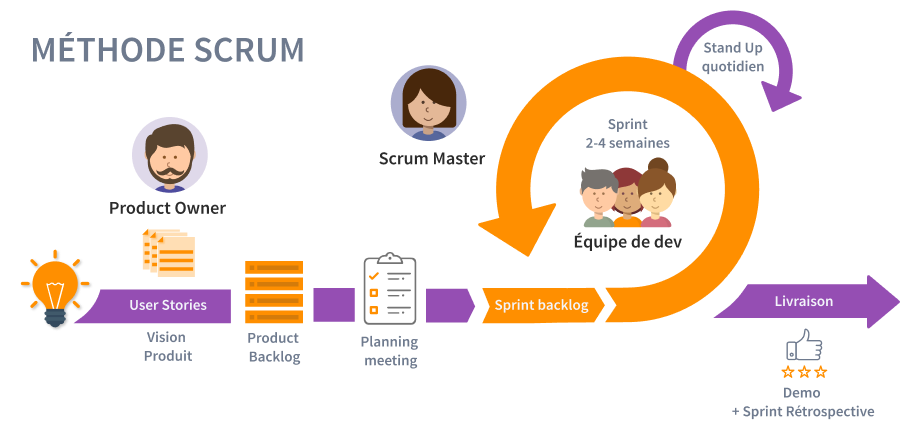
\includegraphics[width=1\textwidth]{logos/scrum.png}
\caption{Présentation du processus SCRUM}
\label{fig:scrum}
\end{figure}

\newpage
\noindent
{\small\textbf{\textit{d. Les rôles de la méthode Scrum :}}}\mbox{} \\
L'adoption de Scrum requiert la mise en place de 3 rôles spécifiques. Il s'agit du: Product owner, de l'équipe de développement et du Scrum master.

\begin{itemize}
  \item \small\textbf{Product Owner: } Le product owner (PO) représente le client ou l'utilisateur final. Son rôle est de veiller à ce que le produit soit conforme aux attentes du client que ce soit en termes de qualité ou de valeur ajoutée.
  
  \item \small\textbf{Scrum Master: } Il est le leader de l'équipe, il s'assure que le scrum est correctement appliquée et respectée et enlève les obstacles qui peuvent perturber l'avancement des travaux.
  
  \item \small\textbf{l'équipe de Développement: } L'équipe de développement est chargée de la mise en œuvre des solutions techniques et de la réalisation des développements requis.
\end{itemize}

\subsection{Le Langage UML}
\noindent
Après le choix de la méthodologie de développement, nous avons besoins d’un langage de modélisation unifiée pour la modélisation de notre projet. Pour concevoir notre système, nous avons choisi UML (Unified Modeling Language) comme un langage de modélisation qui couvre les différents vues du projet. Notre choix s’est basé sur les points forts de ce langage notamment sa standardisation et les divers diagrammes qu’il propose.

\section{Conclusion}
\noindent
Dans ce chapitre, nous avons présenté le cadre général de notre projet en déterminant la problématique et en proposant une solution. Nous avons dévoilé la méthodologie de développement et la méthode de conception qui seront utilisés dans les prochains chapitres de ce rapport et nous avons argumenté notre choix.

\newpage

% L'e-commerce, ou commerce électronique, est une composante essentielle du paysage commercial moderne, révolutionnant la manière dont les entreprises vendent des produits et comment les consommateurs les achètent. Cette forme de commerce implique la vente et l'achat de biens ou de services via Internet, offrant aux consommateurs une commodité sans précédent et aux entreprises une portée mondiale, ainsi que permettre aux entreprises de travailler et d'être ouvertes à prendre des commandes 24h/24

% \noindent
% \begin{itemize}
% \item  \textbf{L'origine de l'e-commerce: } \texttt{}{L'émergence du commerce en ligne est directement liée à l'apparition du web au début des années 1990. Le 11 août 1994, Phil Brandenberger, un habitant de Philadelphie, passe la première commande en ligne en utilisant un système de paiement sécurisé par carte bancaire. \cite{wiki:xxx}}
% \end{itemize}


\chapter{Approches Proposés}
\section{Introduction}
\noindent
Dans cette section en va explorer les différentes solutions potentielles et les différents approches qu'on a pris pour améliorer la recherche dans notre projet. Nous aborderons chacune des technologies utilisés en expliquant leurs fonctions principales, leurs utilisations courantes et leurs avantages. Nous discuterons également de l'importance de ces outils dans le domaine de l'analyse de texte et du traitement du langage naturel. En comprenant ces différentes approches, nous serons en mesure d'explorer en détail leurs fonctionnalités spécifiques et leur pertinence pour notre projet de PFE.

\section{Les solutions possibles}
\noindent
Dans cette section on va explorer les solutions potentielles qu'on peut adopter pour notre projet tel que les différentes techniques de recherches et les bases de donnèes qu'on peut utiliser. 

\subsection{Recherche Régulière}
\noindent
Nous aurions pu utiliser la recherche régulière simplement en faisant correspondre le terme de recherche avec les phrases disponibles dans notre base de données SQL déja existante via des requêtes SQL beaucoup plus optimisés et rapides. Avec cette approche, il y a moins de travail et complexité, mais des résultats beaucoup moins précis.

\subsection{Utilisaton d'une base de donnèes SQL altèrnatif et performante}
\noindent
Nous aurions pu utiliser une différente base de donnèes SQL plus optimisé et performante comme Cassandra pour l'optimisation de vitesse de recherche et la prècision des resultats renvoyès. Avec cette approche la migration des donnèes existantes va être beaucoup plus complexe aussi que l'intègration de cette base de donnèes dans notre application. Mais les rèsultate vont être plus prècis et rapide, mais il reste la limitation la plus importante, qui est la recherche en Arabe avec le dialecte Tunisien, et l'Arabe Traditionnelle. Pour cette raison on a dècidè de prendre l'approche d'Elasticsearch avec le recherche vectorielle qui sont dans les sections ci-dessous.

\section{Recherche Vectorielle}
\noindent
La recherche vectorielle est une approche de la récupération des informations qui prend en charge l’indexation et l’exécution des requêtes sur des représentations numériques du contenu. Étant donné que le contenu est numérique plutôt que texte brut, la correspondance est basée sur des vecteurs qui sont les plus similaires au vecteur de requête, ce qui permet la correspondance entre :
\begin{itemize}
    \item La ressemblance sémantique ou conceptuelle (« chien » et « canine », conceptuellement similaire mais linguistiquement distincte)
    
    \item contenu multilingue (« dog » en anglais et « chien » en Français)
\end{itemize}

\noindent
Pour calculer cette similarité Il y a plusieurs approches de calcul, la plus significante, précis et populaire c'est la similarité cosinus qui utilise cette formule mathématique:
\[\cos(\theta) = \frac{\mathbf{A} \cdot \mathbf{B}}{\|\mathbf{A}\|\|\mathbf{B}\|} = \frac{\sum_{i=1}^{n} A_i B_i}{\sqrt{\sum_{i=1}^{n} A_i^2} \sqrt{\sum_{i=1}^{n} B_i^2}}
\]
Soit $A$ et $B$ deux vecteurs de n'importe quelles dimensions, la similarité cosinus mesure l'angle entre deux vecteurs. Plus l'angle est petit, plus les vecteurs sont similaires, le cosinus de leur angle $\theta$ s'obtient en prenant leur produit scalaire divisé par le produit de leurs normes. Le valeur de cette angle est compris entire [-1, 1], la valeur de -1 indique des vecteurs opposés, la valeur de 0 des vecteurs indépendants (orthogonaux) et la valeur de 1 des vecteurs colinéaires de coefficient positif. Plus que cette valeur s'approche de 1, le plus que les deux vecteurs sont similaires.

\begin{figure}[H]
\centering
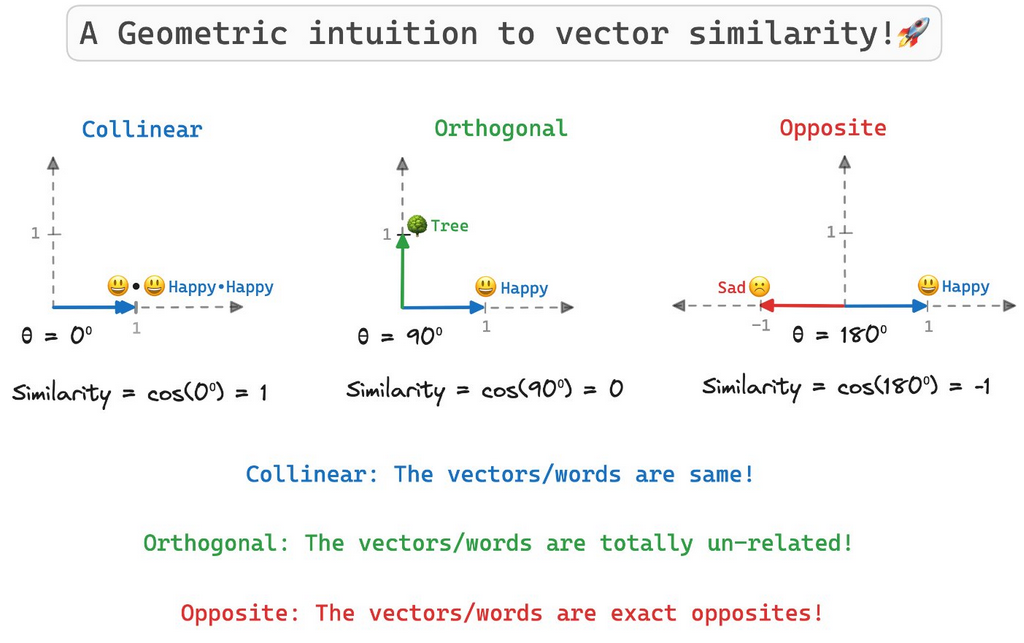
\includegraphics[width=1\textwidth]{logos/cosine.png}
\caption{Présentation du similarité cosinus}
\label{fig:cosine}
\end{figure}

\section{Elasticsearch}
\noindent
Elasticsearch est un outil d'analyse de donnèes distribuès open source et hautement èvolutif. Il est conçu pour stocker, rechercher et analyser et rechercher de grands volumes de données de manière rapide et efficace en utilisant des diffèrents mèthodes comme Knn Search.
Il utilise une structure de données de type index inversé pour indexer et rechercher rapidement des documents. Il prend en charge une variété de types de données, notamment le texte, les nombres, les dates, et les vecteurs par exemple le type dense vector. Avec tout sa, Elasticsearch facilite et optimise la recherche sémantique(vectorielle) en utilisant des indices inversés qui nous permet de stocker des données de type dense vector (vecteur), qui sont extrêmement efficaces pour la recherche de texte complet. Au lieu de parcourir chaque document et de vérifier la correspondance avec les termes de la requête, Elasticsearch utilise cet indice inversé pour trouver rapidement les documents contenant les termes de recherche. Cela accélère considérablement le processus de recherche, car l'indice fonctionne comme un système de référence rapide.

\section{Utilisation d'un modéle Sentence-Transformers}
\noindent
Notre modéle de choix est un modéle appelé << all-mpnet-base-v2 >> qui est basé sur le modèle mpnet-base de Microsoft, et puisqu'il est déja pré-entraînée pour comprendre la langue Française. Il sert a convertir des des phrases et des paragraphes en vecteurs sémantiques de 768 dimensions dans un espace vectoriel, avec une limite des paragraphes de 384 mots au maximum. Il est spécifiquement affiné pour établir des correspondances sémantiques précises entre les phrases en les plaçant dans un espace où la similarité cosinus peut être calculée efficacement pour des tâches comme la recherche sémantique, et la mesure de la similarité des phrases. \\
\citetitle{pinecone:mpnet} (\cite{pinecone:mpnet})

\subsection{Comment le modéle intérpréte les phrases?}
\noindent
Pour interpréter les phrases, le modéle est besoin d'un << Tokenizer >> puisqu'il ne peux pas comprendre du texte, on doit convertir chaque phrase en une représentation numérique. Le processus est appelé la << tokenisation >> qui est le processus de conversion d'une séquence de caractères en une séquence de jetons(tokens). En PNL, un jeton(token) représente généralement un mot, mais il peut également représenter des sous-mots, des caractères ou d'autres unités, selon le tokeniseur. Ce processus est nécessaire car notre modèle ne peux pas comprendre le texte brut. Au lieu de cela, il travail avec des représentations numériques de jetons. La figure ~\ref{fig:paddingexplanation} présente le processus de tokenisation.

\begin{figure}[H]
\centering
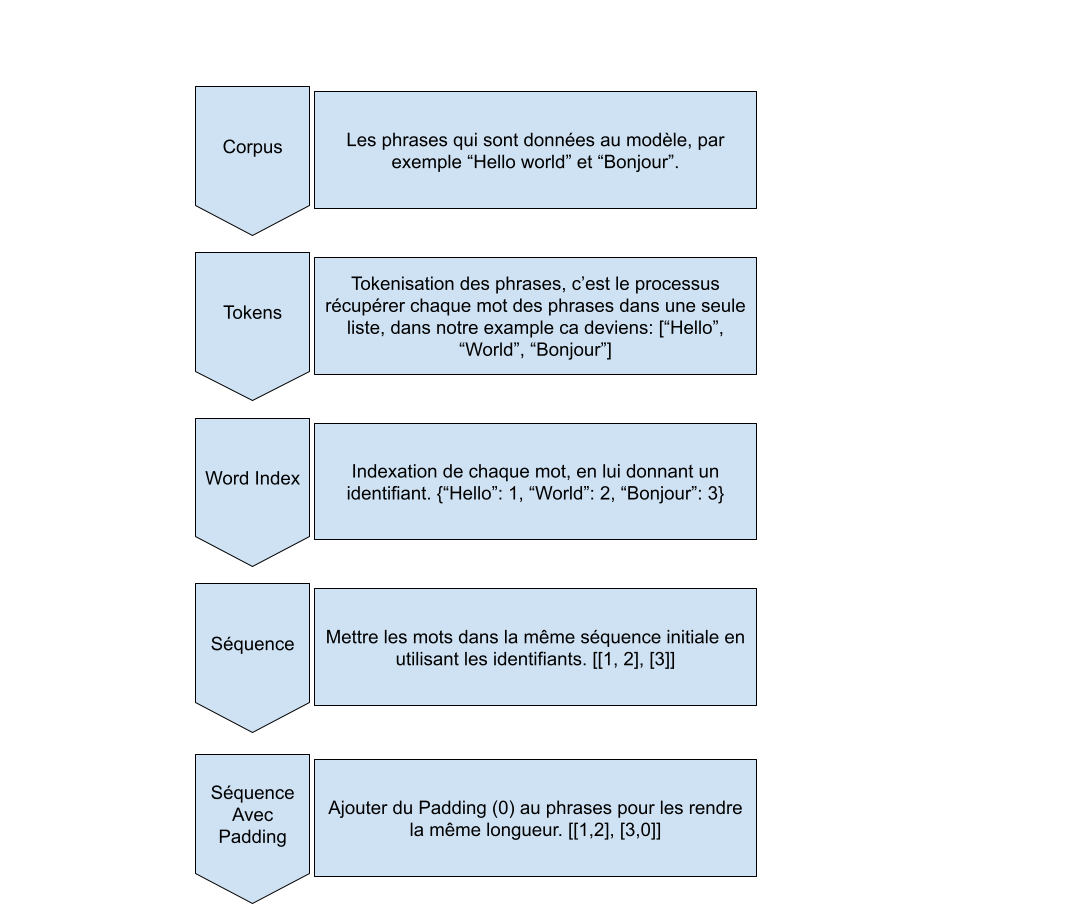
\includegraphics[width=1\textwidth]{logos/paddingexplanation.png}
\caption{Presentation du processus de tokenisation}
\label{fig:paddingexplanation}
\end{figure}

\noindent
La figure ~\ref{fig:padding} présente un exemple du processus de tokenisation.

\begin{figure}[H]
\centering
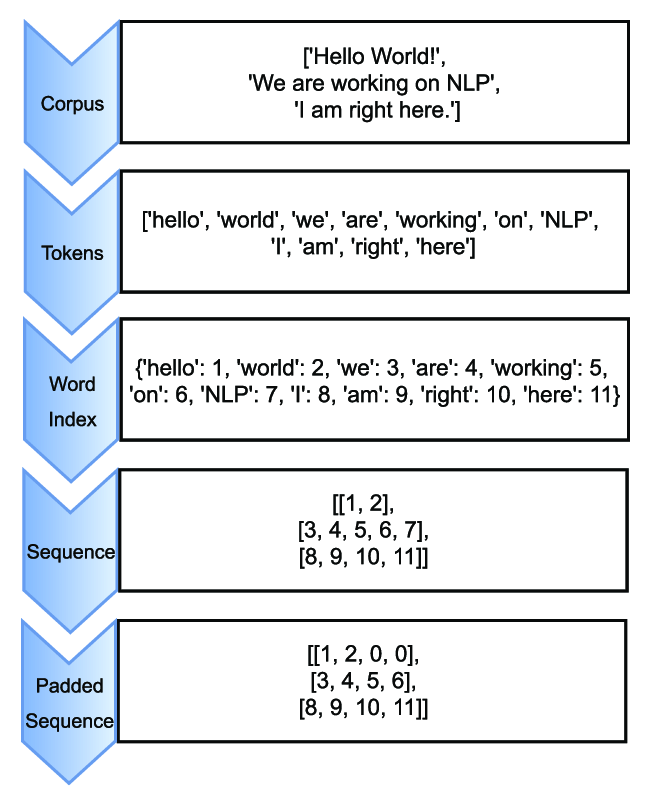
\includegraphics[width=1\textwidth]{logos/padding.png}
\caption{Exemple du processus de tokenisation}
\label{fig:padding}
\end{figure}

\newpage
\noindent
{\small\textbf{\textit{a. Padding }}}\mbox{}\\
Le remplissage(padding) est appliqué pour garantir que toutes les séquences d'un lot ont la même longueur, ce qui est une exigence pour de nombreuses architectures de réseaux neuronaux. Des jetons de remplissage sont ajoutés à la fin de la séquence pour étendre sa longueur jusqu'à un maximum prédéfini, qui est de 384 dans notre cas.

\noindent
{\small\textbf{\textit{b. Attention Mask (Masque d'attention) }}}\mbox{}\\
C'est simplement un masque qui fait la différence entre le contenu et les jetons de remplissage.

\noindent
{\small\textbf{\textit{c. Mean Pooling (Regroupement des moyennes) }}}\mbox{}\\
C'est un processus qui calcule efficacement la moyenne de la sequence obtenu aprés le padding tout en ignorant les jetons de remplissage (padding tokens) qui ont une valeur de 0, ce qui donne un seul vecteur d'intégration qui représente la phrase entière.
Ce processus ne prend en compte que les jetons sans remplissage dans la phrase, en utilisant un masque d'attention. Le masque d'attention a la même longueur que la séquence de jetons, « 1 » indiquant les jetons sans remplissage et « 0 » pour les jetons de remplissage. Cela garantit que l'incorporation de phrase résultante est calculée uniquement à partir du contenu significatif de la séquence. La figure ~\ref{fig:meanpooling} présente ce processus.

\begin{figure}[H]
\centering
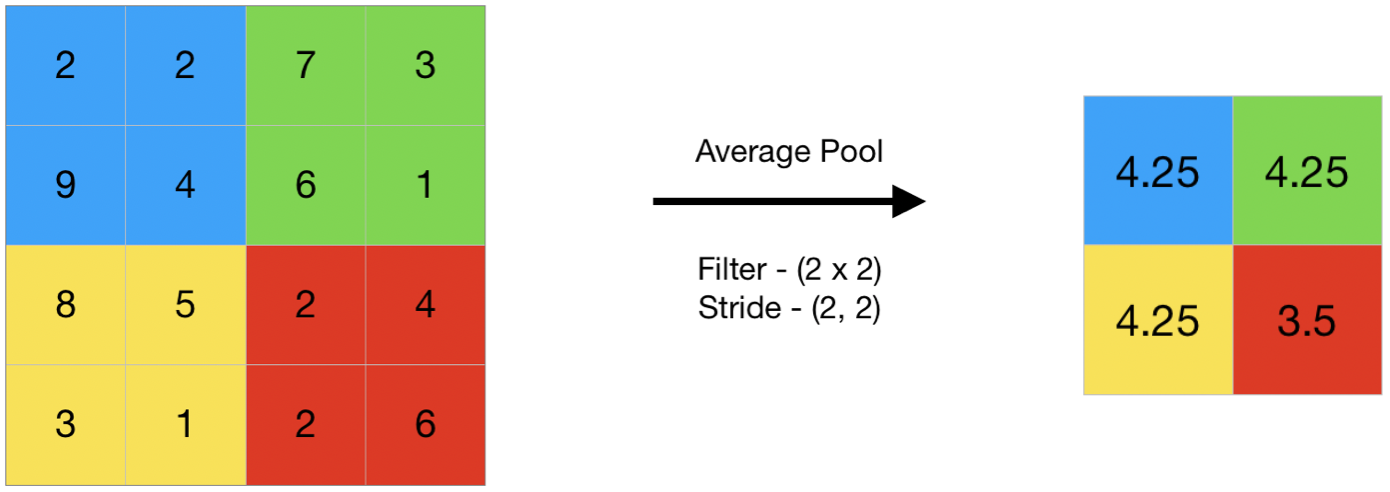
\includegraphics[width=1\textwidth]{logos/mean_pooling.png}
\caption{Présentation du processus de Mean Pooling}
\label{fig:meanpooling}
\end{figure}

\subsection{Pourquoi utiliser Mean Pooling plutôt qu'un autre type de pooling?}
\noindent
Puisque notre modéle génère un vecteur pour chaque token aprés les étapes précédentes, le mean pooling consiste à prendre la moyenne de ces vecteurs sur tous les tokens, ce qui résulte en un unique vecteur qui est censé capturer l'essence sémantique de l'ensemble de la phrase, et donner importance à tous les mots de phrase, tous en nous permettant de prendre et interpréter le contexte de toute la phrase. Il existe deux autres types do pooling qu'on a testé sans obtenir de résultats aussi bons:

\noindent
{\small\textbf{\textit{a. Max Pooling }}}\mbox{}\\
Ce processus consiste à prendre la valeur maximum de ces vecteurs sur tous les tokens au lieu de la moyenne. La probléme avec cette stratégie est ce que elle peut donner plus importance à une mot ou phrase plus que les autres et alterner les résultats de manière négative, ce qui entraîne moins de précision. Par exemple, si un personne cherche pour un << T-shirt bleu >>, avec le max pooling, le mot << bleu >> peut avoir plus d'importance que t-shirt, donc il peut retourner tous les produits bleus, au lieu des t-shirts. La figure ~\ref{fig:maxpooling} présente ce processus. 

\begin{figure}[H]
\centering
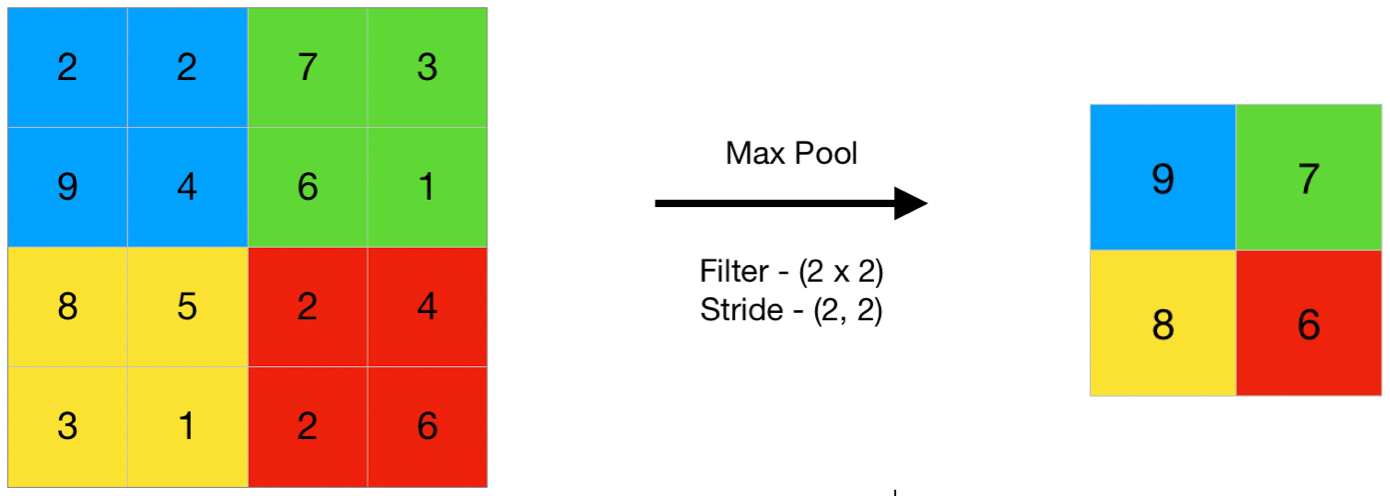
\includegraphics[width=1\textwidth]{logos/max_pooling.png}
\caption{Présentation du processus de Max Pooling}
\label{fig:maxpooling}
\end{figure}

\newpage
\noindent
{\small\textbf{\textit{b. Min Pooling }}}\mbox{}\\
Ce processus consiste à prendre la valeur minimum de ces vecteurs sur tous les tokens au lieu de la moyenne. La probléme avec cette stratégie est ce que elle peut donner moins importance à une mot ou phrase clé moins que les autres et alterner les résultats de manière négative, ce qui aussi entraîne moins de précision. Prenant le même exemple précédent, si un personne cherche pour un << T-shirt bleu >>, avec le min pooling, le mot << bleu >> peut avoir moins d'importance que t-shirt, donc il peut retourner tous les t-shirts sauf les bleus. La figure ~\ref{fig:minpooling} présente ce processus. 

\begin{figure}[H]
\centering
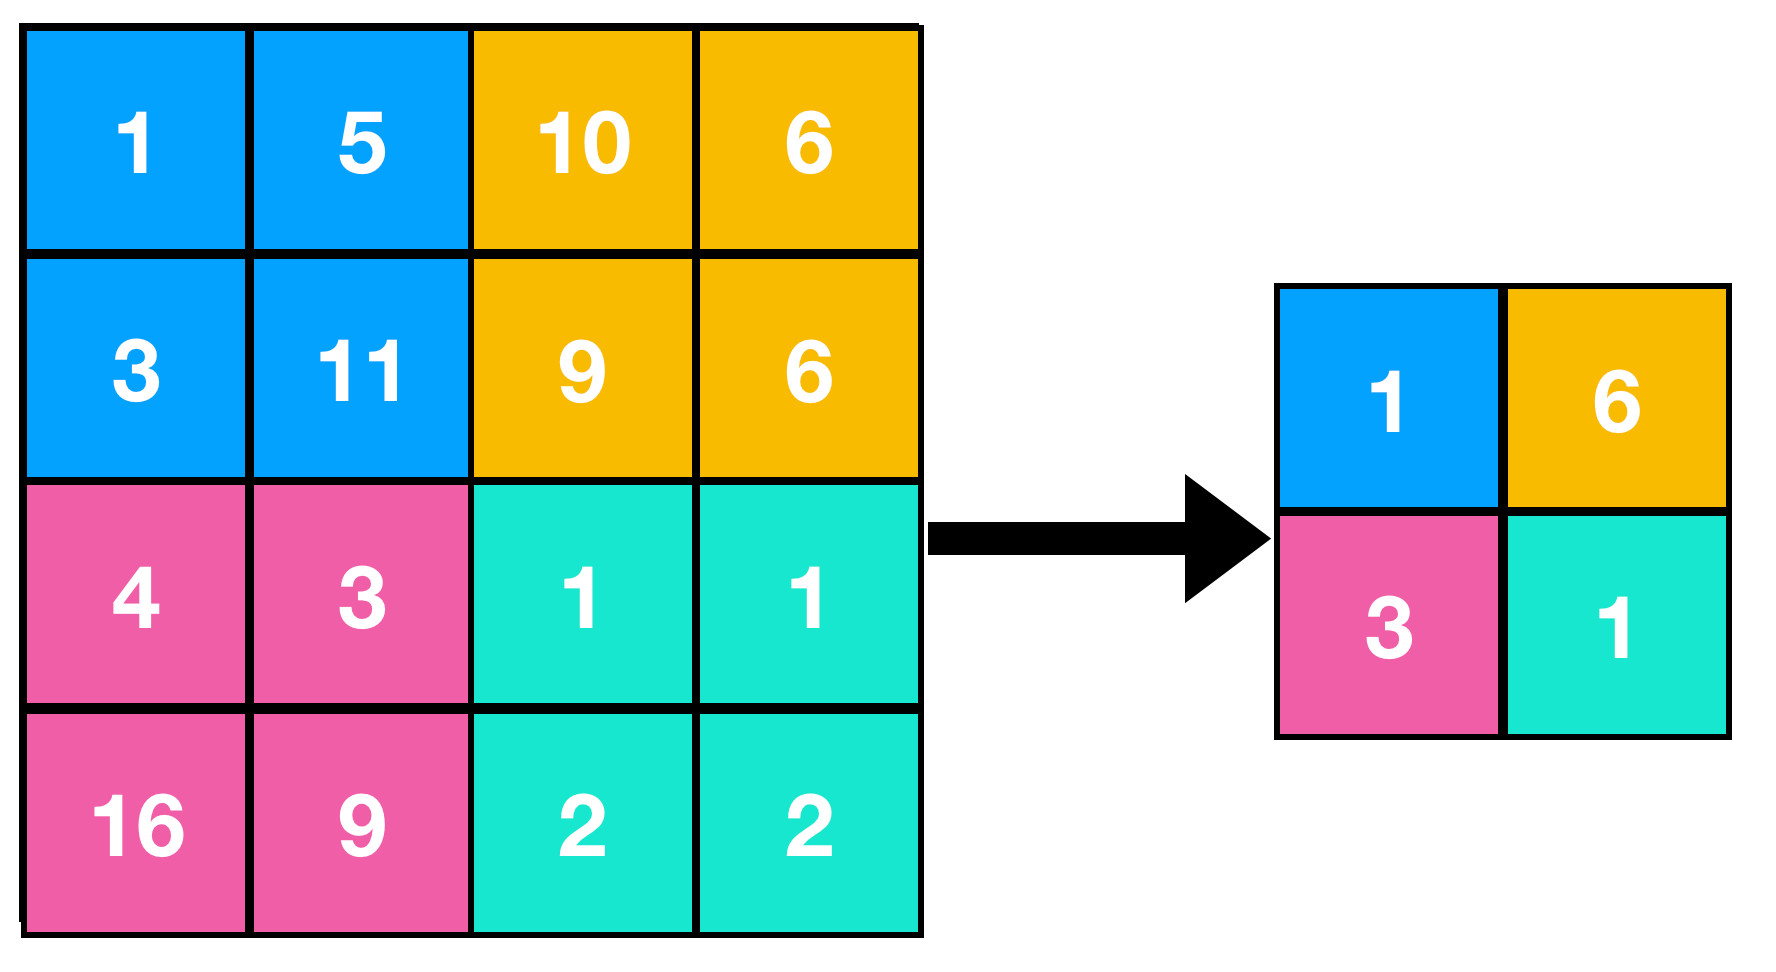
\includegraphics[width=1\textwidth]{logos/min_pooling.png}
\caption{Présentation du processus de Min Pooling}
\label{fig:minpooling}
\end{figure}


\section{Conclusion}
\noindent
Dans cette section on a presenté et expliqué les approches qu'on a décidé de prendre ainsi que les technologies qu'on a utilisé et leurs importance, pertinence et les benéfices qu'ils apportent a notre projet tels que le Recherche Vectorielle, l'Elasticsearch et le modéle sentence-transformers.
\chapter{Sprint 0: Planification du projet}
\etocsettocstyle{\section*{Sommaire}}{}
\localtableofcontents
\section{Introduction}
\noindent
Dans ce chapitre, on va présenter la premiére phase de la méthode SCRUM, qui est le Sprint 0, qui commence par l'identification des besoins. Par la suite, nous faisons une analyse globale de notre projet en identifiant les acteurs et ensuite le diagramme de cas d'utilisation globale. De plus, nous planifions le reste des sprints de notre projet. Puis, on va présnter l'architecture du systéme pour laquelle nous avons opté. Et enfin, on va présenter les outils de développement utilisés pour réaliser ce projet.

\section{Identification des besoins}
\subsection{Les besoins fonctionnels}
\noindent
Les besoins fonctionnels sont les fonctionnalités que le systéme doit livrer aux utilisateurs.
L’outil n’est considéré comme opérationnel que si sa disponibilité fonctionnelle est garantie.
Dans le cas du notre systéme, ces besoins se concentrent sur:

\begin{itemize}
    \item \small\textbf{Vitesse de recherche: } {Améliorer les vitesses de recherche au maximum afin de renvoyer des résultats précis au client.}
    
    \item \small\textbf{Recherche en Français: } {Permettre le client a rechercher les produits dans la langage Française.}

    \item \small\textbf{Recherche en Arabe Tunisienne: } {Permettre le client a rechercher les produits dans la langage Arabe Tunisienne.}

    \item \small\textbf{Recherche en Arabe Traditionnel: } {Permettre le client a rechercher les produits dans la langage Arabe Classique.}
    
    \item \small\textbf{Suggestion des produits: } {Si le produit recherché par le client n'existe pas, le système tentera de suggérer des produits similaires en prenant le contexte du terme de recherche.}
\end{itemize}

\newpage
\subsection{Les besoins non fonctionnels}
\noindent
Les exigences non fonctionnels décrivent les objectifs liés aux performances du systéme et d'autres aspects cruciaux du système qui ne sont pas directement liés à ses fonctionnalités spécifiques. Ils définissent les critères de qualité que le système doit respecter pour répondre aux attentes des utilisateurs. Notre systéme doit repondre aux exigences non fonctionnels suivantes:

\begin{itemize}
    \item \small\textbf{La Fiabilité: } L'application doit être fonctionnelle sans détection des erreurs afin de satisfaire les besoins de client.

    \item \small\textbf{La Sécurité: } Vu que l'application contient des données confidentielles, tous l'accés des produits doivent être protégées par un privilege d'accées.

     \item \small\textbf{La Disponibilité: } Les services offerts par notre application sont disponibles pendant les 24
     heures et durant toute la semaine.

     \item \small\textbf{La Performance: } L'application doit être rapide et robuste (Vitesse de réponse rapide et précision des résultats lors du recherche des produits dans les langues différents).
\end{itemize}

\newpage
\section{Diagramme de cas d’utilisation global}
\subsection{Introduction}
\noindent
Dans cette partie, on va présenter les besoins de notre systéme de façon formelle à l'aide du diagramme de cas d'utilisation du langage de modélisation UML. D'abord nous identifions les acteurs qui intéragissent avec notre systéme, qui sont:

\noindent
\small\textbf{Le Visiteur: } C'est le personne qui va accéder à notre systéme pour rechercher le(s) produit(s) dans notre systéme.

\noindent
\small\textbf{Le Client: } C'est aussi le personne qui va accéder à notre systéme pour rechercher le(s) produit(s) de ses besoins. 

\noindent
\small\textbf{L'Admin: } C'est le personne qui va accéder à notre systéme pour rechercher le(s) produit(s) dans notre systéme et modifier les paramétres de son recherche. 

\begin{figure}[H]
\centering
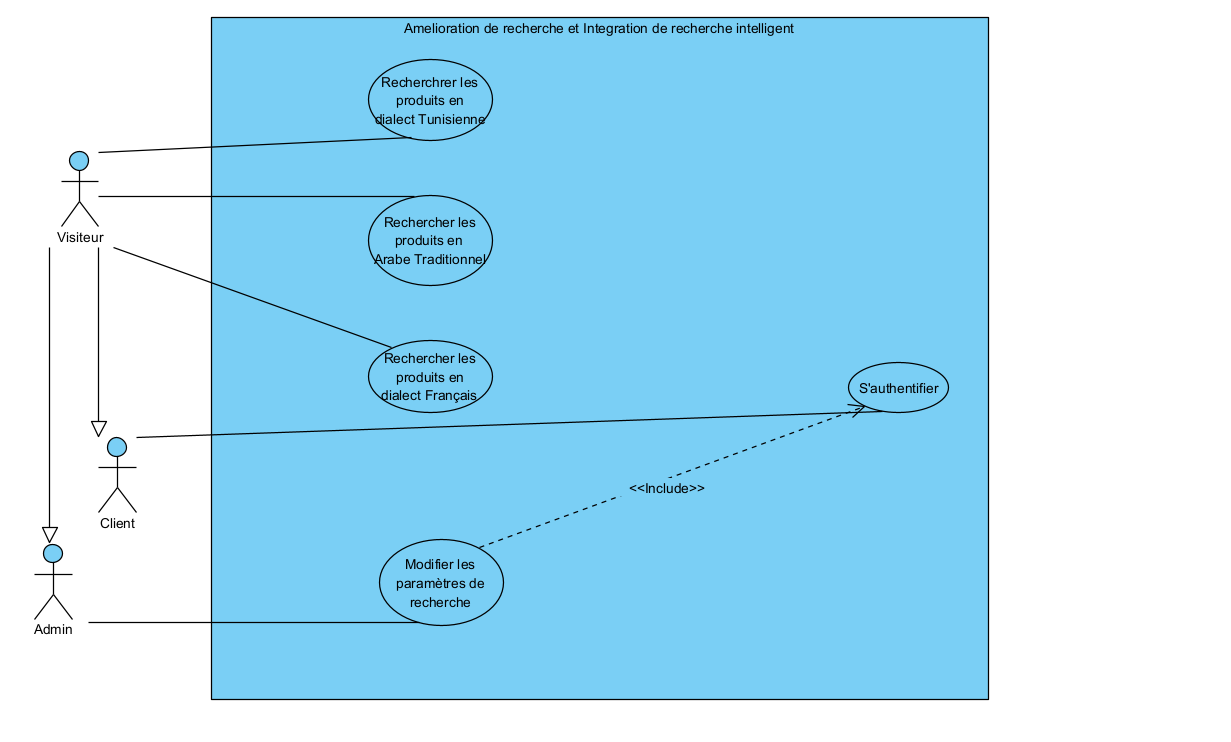
\includegraphics[width=1\textwidth]{logos/CU_global.png}
\caption{Présentation de Diagramme de Cas D'Utilisation global}
\label{fig:diagcuglobal}
\end{figure}
\section{Backlog De Produit}
\noindent
\large
Le backlog de produit est une liste de fonctionnalités à réaliser. Ces fonctionalités sont exprimées sous formes des besoins et sont priorisées par le Product Owner ce qui permet d'établir un ordre de réalisation à respecter. \\
Notre backlog est composé de trois colonnes: \\
\textbf{ID: } C'est l'identifiant du scénario \\
\textbf{Fonctionnalité: } Permet de mieux ordonner les scénarios. \\
\textbf{Scénario: } Comporte la description des scénarios suivant le forme << En tant que ... Je veux >> \\

\begin{table}[H]
\centering
\begin{tabular}{|c|c|p{10cm}|}
\hline
\rowcolor{blue!20}
\textbf{ID} & \textbf{Fonctionnalité} & \textbf{Scénario} \\ \hline
1 & Recherche en Arabe Tunisienne  & En tant qu'un client, je veux rechercher un ou plusieurs produits dans la langue Tunisienne. \\ \hline
2 & Recherche en Arabe Classique & En tant qu'un client, je veux rechercher un ou plusieurs produits en Arabe Classique. \\ \hline
3 & Recherche en Français & En tant qu'un client, je veux rechercher un ou plusieurs produits en Français. \\ \hline
4 & Vitesse de recherche & En tant qu'un client, je veux avoir une vitesse de recherche rapide. \\ \hline
5 & Suggestion des produits & En tant qu'un client, si le produit que je cherche n'existe pas, je veux avoir des suggestions des produits similaires. \\ \hline
\end{tabular}
\caption{Table des fonctionnalités et scénarios.}
\end{table}
\section{La Plannification De Release}
\noindent
Une fois que le Product Owner a fini de construire le Product Backlog, l'équipe SCRUM et l'environnement technique du projet est bien mis en œuvre, et tous le membres du projet sont plannifiés le sprint ensemble aussi que les fonctionnalités à développer pour chaque Sprint, la durée de la prévision de chaque sprint est estimée à quatre semaines.
\section{Architecture du systéme}
\noindent
Il est indispensable à la conception de tout systéme informatique de choisir le modéle d'architecture adéquat et pourra assurer le bon fonctionnement, une meilleure performance, ainsi que la scalabilité, la fiabilité et trés important, la productivité de développement. \\
C'est pour cette raison, qu'on a opté pour l'architecture MVC avec des microservices (Modèle, Vue, Contrôleur, Modèle IA, et Elasticsearch) comme l'architecture global du projet, et le modèle << Clean Architecture >>, dans le backend, qui seront trés pratique pour gérer les intéractions entre les différents composants de notre application. Nous décrirons ces architectures dans les prochaines sections.

\subsection{Architecture "MVC Avec Microservices"}
\noindent
Le modèle MVC permet de bien organiser son code source. Il va nous aider à savoir quels fichiers créer, mais surtout à définir leur rôle. Le but de MVC est justement de séparer la logique du code en trois parties que l'on retrouve dans des fichiers distincts.

\noindent
{\small\textbf{\textit{Modèle}}}\mbox{}\\
Cette partie gère ce qu'on appelle la logique métier de notre site. Elle comprend notamment la gestion des données qui sont stockées, mais aussi tout le code qui prend des décisions autour de ces données. Son objectif est de fournir une interface d'action la plus simple possible au contrôleur. On y trouve donc entre autres des algorithmes complexes et des requêtes SQL, et Elasticsearch dans notre cas.

\noindent
{\small\textbf{\textit{Vue}}}\mbox{}\\
Cette partie se concentre sur l'affichage. Elle ne fait presque aucun calcul et se contente de récupérer des variables pour savoir ce qu'elle doit afficher. On y trouve essentiellement du code HTML mais aussi quelques boucles et conditions Javascript très simples, pour afficher par exemple une liste de messages. Il est développé avec React et Typescript.

\noindent
{\small\textbf{\textit{Contrôleur}}}\mbox{}\\
Cette partie gère les échanges avec l'utilisateur. C'est en quelque sorte l'intermédiaire entre l'utilisateur, le modèle et la vue. Le contrôleur va recevoir des requêtes de l'utilisateur. Pour chacune, il va demander au modèle d'effectuer certaines actions (demander les produits en fonction d'un mot-clé de recherche) et de lui renvoyer les résultats (la liste des produits). Puis il va adapter ce résultat et le donner à la vue. Enfin, il va renvoyer la nouvelle page HTML, générée par la vue, à l'utilisateur. Il est implémenté avec ASP .NET Core et C\# et utilise des requêtes SQL et Elasticsearch pour manipuler les donnèes.

\noindent
{\small\textbf{\textit{Modèle IA}}}\mbox{}\\
Notre modèle IA a une et une seule responsabilité, qui est de faire l'encodage de la requête de l'utilisateur qui est envoyé au contrôleur et retourner le résultat encodé.

\noindent
{\small\textbf{\textit{Elasticseach}}}\mbox{}\\
Elasticsearch agit comme notre base de données de recherche de vecteurs qui contient notre index de produits contenant 2 colonnes de vecteurs recherchables à l'aide du vecteur codé renvoyé par le modèle AI.

\newpage
\noindent
La figure ~\ref{fig:mvc} schématise le rôle de chacun de ces éléments.
\begin{figure}[H]
\centering
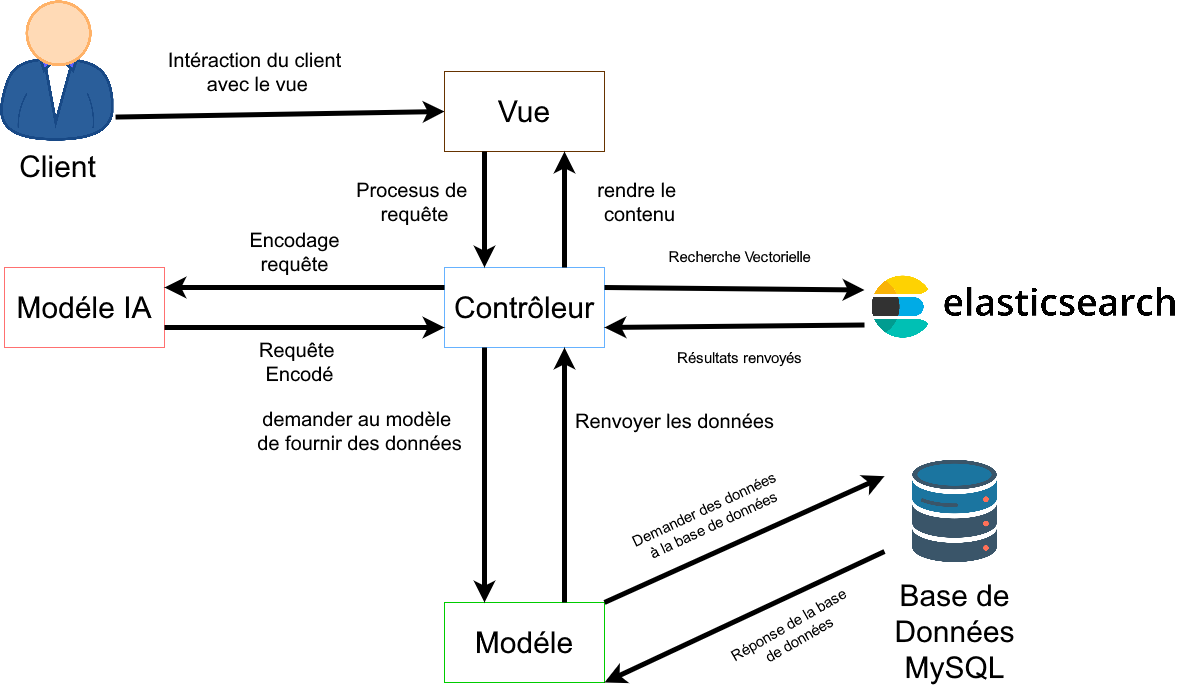
\includegraphics[width=1\textwidth]{logos/mvcavecservice.png}
\caption{L'architecture MVC avec microservices}
\label{fig:mvc}
\end{figure}

\noindent
Il est important de bien comprendre comment ces éléments s'agencent et communiquent entre eux. La figure ~\ref{fig:mvcechange} montre cette communication.

\begin{figure}[H]
\centering
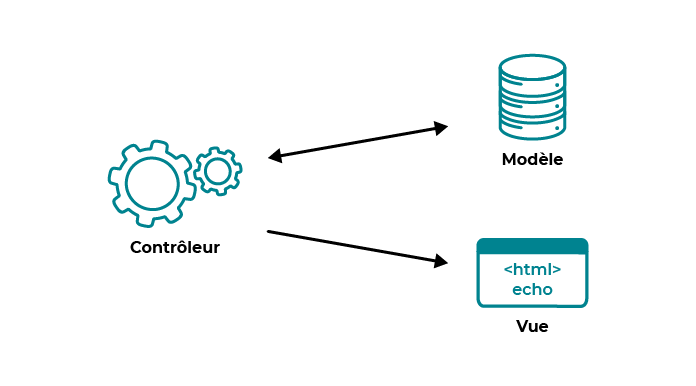
\includegraphics[width=1\textwidth]{logos/mvcechange.png}
\caption{Échange d'informations entre les éléments MVC}
\label{fig:mvcechange}
\end{figure}

\subsection{Architecture "Clean Architecture"}
\noindent
"Clean Architecture" est un modèle architectural introduit par Robert C. Martin, également connu sous le nom d'Oncle Bob. Il favorise une séparation claire des préoccupations en divisant l'application en couches concentriques, chaque couche ayant ses responsabilités et ses dépendances. Le principe fondamental derrière l'architecture propre est la règle de dépendance, qui stipule que les dépendances doivent toujours pointer vers l'intérieur vers les couches les plus stables et abstraites, plutôt que vers l'extérieur vers des couches plus concrètes et volatiles. 

\noindent
Cette architecture se compose généralement des couches suivantes: \\

\begin{itemize}
    \small\item \textbf{La couche Presentation: } Cette couche est responsable de la gestion des interactions des utilisateurs et de la fourniture des données à l'interface utilisateur. Dans notre context d'une API Web .NET Core, cette couche comprend les contrôleurs et autres composants qui gèrent les requêtes et les réponses HTTP.

    \small\item \textbf{La couche Application: } La couche Application contient la logique métier et les cas d’utilisation de l’application. Il agit comme intermédiaire entre la couche présentation et la couche domaine. Cette couche est indépendante de tout problème spécifique d’interface utilisateur ou d’infrastructure.
    \small\item \textbf{La couche Domain: } La couche Domain représente le noyau de l’application, encapsulant les règles métier, les entités, les interfaces (Orienté Objet) des repositories des bases de donnés et la logique spécifique au domaine. Il doit être indépendant de la technologie et ne contenir aucune dépendance vis-à-vis de frameworks ou de bibliothèques externes.

    \small\item \textbf{La couche Infrastructure: } La couche infrastructure traite des problèmes externes tels que les bases de données, les services externes et les frameworks. Il contient des implémentations d'interfaces définies dans la couche application et interagit avec des ressources externes.
\end{itemize}

\noindent
La figure Figure~\ref{fig:architecture} reprèsente les couches de << Clean Architecture >>

\begin{figure}[H]
\centering
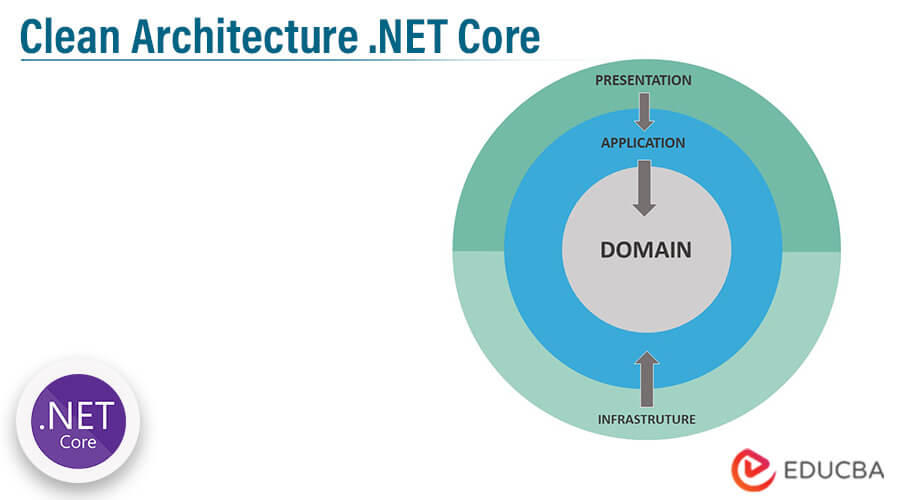
\includegraphics[width=1\textwidth]{logos/clean_architecture.png}
\caption{Architecture "Clean Architecture" dans ASP. NET Core}
\label{fig:architecture}
\end{figure}

\noindent
Les avantages de l’utilisation de  << Clean Architecture >> :

\begin{itemize}[label={---}]
    \item \small\textbf{Vitesse d'implementation: } La mise en œuvre immédiate vous permet d'implémenter cette architecture avec n'importe quel langage de programmation.

    \item \small\textbf{Les couches de Domain et Application comme noyau du système}: Les couches Domain et Application sont toujours au centre de la conception et sont connus comme le cœur du système, c'est pourquoi le cœur du système ne dépend pas de systèmes externes. 

    \item \small\textbf{Indépendence des systémes externes: } Cette architecture permet de changer de système externe sans affecter le cœur du système.

    \item \small\textbf{Testabilité améliorée du code: } Dans un environnement qui depends hautement des tests(unitaires et d'intégration), vous pouvez tester votre code rapidement et facilement.    

    \item \small\textbf{Création de produits scalables, robustes et de haute qualité: } Vous pouvez vitement créer un systéme bien performant, organisé, testable, scalable, et robuste.
\end{itemize}
\noindent
\section{L'environnement de développement et choix techniques: }

\subsection{Introduction}
\noindent
Le développement de notre projet nécessite un ordinateur avec des spécifications puissantes en raison de choses telles que le développement de C\# dans Visual Studio, le lancement des containers Docker, le lancement et le stockage de données dans Elasticsearch, l'importation et l'utilisation de notre modèle Sentence-Transformers, et surtout l'exécution de la recherche vectorielle. C'est pour cette raison que nous disposons d'ordinateurs avec les spécifications mentionnées dans la section  de l'environnement matériel ci-dessous. \\
\citetitle{elastic:hardwarespecifications} (\cite{elastic:hardwarespecifications})

\subsection{L'environnement matériel}
\noindent
Dans la table~\ref{tab:compspec} nous mentionnons les spécifications des ordinateurs utilisés pour le développement de notre application: 

\begin{table}[H]
\centering
\begin{tabular}{|c|c|c|c|}
\hline
\rowcolor{blue!20}
\textbf{Processeur} & \textbf{Mémoire} & \textbf{Disque dur} & \textbf{Système d'exploitation} \\
\hline
11th Gen Intel Core i7 @ 2.304GHz & 32Go & 1.5To SSD & Windows 11-64bits \\
\hline
9th Gen Intel Core i7 @ 1.8GHz & 32Go & 1To SSD 1To HDD & Windows 10-64bits \\
\hline
\end{tabular}
\caption{Spécifications des ordinateurs utilisés}
\label{tab:compspec}
\end{table}

\newpage
\subsection{L'environnement logiciel}
\noindent
{\small\textbf{\textit{Visual Studio}}}\mbox{}\\
Visual Studio est un environnement de développement intégré (IDE) créé par Microsoft. Il est principalement utilisé pour le développement de logiciels, notamment pour les langages de programmation tels que C\#, C++. Pour C\# il offre beacoup des outils qui aide et accélére et améliore l'expérience de développement comme une complétion automatique intelligente, création des classes/interfaces intelligente et un débogeur puissant pour détecter et résoudre les erreurs. La figure ~\ref{fig:vs} présente le logo de Visual Studio.

\begin{figure}[H]
\centering

\includegraphics[width=0.3\textwidth]{logos/vs.png}
\caption{Logo officiel du logiciel Visual Studio}
\label{fig:vs}
\end{figure}

\noindent
{\small\textbf{\textit{Visual Studio Code}}}\mbox{}\\
Visual Studio Code (VS Code) est un éditeur de code source gratuit et open source développé par Microsoft connu par sa légèreté, rapidité et personnalisation à travers les extensions qu'il fournit pour une diversité des langages de programmation.
Il fournit beaucoup de choses qu'un IDE fait comme la coloration syntaxique, la complétion automatique, et le déboggage, et la gestion de versions intégré. La figure ~\ref{fig:vsc} présente le logo de Visual Studio Code.
\begin{figure}[H]
\centering

\includegraphics[width=0.3\textwidth]{logos/vsc.png}
\caption{Logo officiel du logiciel Visual Studio Code}
\label{fig:vsc}
\end{figure}

\noindent
{\small\textbf{\textit{C\#}}}\mbox{}\\
C\# (prononcé "C sharp") est un langage de programmation de haut niveau, orienté objet, développé par Microsoft dans le cadre de sa plateforme .NET. Lancé en 2000, C\# a été conçu pour être simple, moderne, sûr et évolutif. C\# est utilisé pour le développement  d'une variété des applications, nottament des applications backend et des REST API web avec ASP .NET Core. La figure ~\ref{fig:cs} présente le logo de C\#.
\begin{figure}[H]
\centering

\includegraphics[width=0.3\textwidth]{logos/csharp.png}
\caption{Logo officiel du langage de programmation C\#}
\label{fig:cs}
\end{figure}

\noindent
{\small\textbf{\textit{ASP .NET Core}}}\mbox{}\\
ASP.NET Core est un framework open source développé par Microsoft pour la création d'applications web modernes. Il constitue la prochaine évolution de la plateforme ASP.NET, offrant une architecture modulaire, légère et hautement performante. Il offre une large flexibilité et une modularité au développeurs, il prend en charge principalement le développement des APIs web RESTful qui peuvent être déployé sur Windows, Linux et MacOS. Il offre une variété des fonctionallités comme le traitement asynchrone des requêtes, le middleware et le pipeline de requêtes personnalisable.
la figure ~\ref{fig:netcore} présente le logo de ASP .NET Core.
\begin{figure}[H]
\centering

\includegraphics[width=0.3\textwidth]{logos/dotnetcore.png}
\caption{Logo officiel du framework ASP .NET Core}
\label{fig:netcore}
\end{figure}

\noindent
{\small\textbf{\textit{Python}}}\mbox{}\\
Python est un langage de programmation interprété, de haut niveau, polyvalent puisqu'il est utilisé dans plusieurs domaines notamment l'analyse de données et le machine learning (avec des bibliothèques telles que NumPy, Pandas, et PyTorch). La figure ~\ref{fig:py} présente le logo de Python.
\begin{figure}[H]
\centering

\includegraphics[width=0.3\textwidth]{logos/pypng.png}
\caption{Logo officiel du langage de programmation Python}
\label{fig:py}
\end{figure}

\noindent
{\small\textbf{\textit{Jupyter Notebook}}}\mbox{}\\
Jupyter Notebook est une application web open source qui permet de créer et de partager des documents interactifs contenant du code qui sont composés des cellules de code qui peuvent être exécuté individuellement, et facilement partagé à travers des differents sites comme Kaggle, Google Collab. La figure ~\ref{fig:jupyter} présente le logo de Jupyter.
\begin{figure}[H]
\centering

\includegraphics[width=0.3\textwidth]{logos/jupyter.png}
\caption{Logo officiel du framework Jupyter}
\label{fig:jupyter}
\end{figure}


\noindent
{\small\textbf{\textit{Flask}}}\mbox{}\\
Flask est un framework Python trés minimalistique pour développer des REST APIs en Python. Il est très facile de configurer et de faire fonctionner une API. Et pour cette raison, nous l'avons utilisé pour exposer un point de terminaison d'API REST unique afin d'exposer notre modèle Sentence-Transformers. La figure ~\ref{fig:flask} présente le logo de Flask.
\begin{figure}[H]
\centering

\includegraphics[width=0.3\textwidth]{logos/flask.png}
\caption{Logo officiel du framework Flask}
\label{fig:flask}
\end{figure}


\noindent
{\small\textbf{\textit{React}}}\mbox{}\\
React est un framework Javascript gratuit et open-source développé et maintenu par méta(anciennement sous le nom Facebook) en 2013 utilisée principalement pour le développement des interfaces utilisateurs web complexes à travers des "components", ou composants en Français. La figure ~\ref{fig:react} présente le logo de React.
\begin{figure}[H]
\centering

\includegraphics[width=0.3\textwidth]{logos/react.png}
\caption{Logo officiel du bibilothéque React}
\label{fig:react}
\end{figure}

\noindent
{\small\textbf{\textit{Typescript}}}\mbox{}\\
Typescript est un langage de programmation gratuit et open-source développé et maintenu par Microsoft principalement pour améliorer l'expérience de développement pour les développeurs Javascript en fournisaant des types statiques, des erreurs directement dans l'éditeur de code, et support totale pour la programmation Orienté Objet. La figure ~\ref{fig:typescript} présente le logo de Typescript.
\begin{figure}[H]
\centering

\includegraphics[width=0.3\textwidth]{logos/typescript.png}
\caption{Logo officiel du langage Typescript}
\label{fig:typescript}
\end{figure}

\noindent
{\small\textbf{\textit{Docker}}}\mbox{}\\
Docker est une plateforme open source qui permet de développer, de déployer et d'exécuter des applications de manière efficace en utilisant des conteneurs logiciels. Les conteneurs sont des unités d'exécution légères et autonomes qui encapsulent une application et tous ses composants, y compris les bibliothèques, la version de langages de programmation utilisè(s), les ports exposès... 
la figure ~\ref{fig:docker} prèsente le logo de Docker.
\begin{figure}[H]
\centering

\includegraphics[width=0.3\textwidth]{logos/docker.png}
\caption{Logo officiel du Docker}
\label{fig:docker}
\end{figure}

\noindent
{\small\textbf{\textit{Elasticsearch}}}\mbox{}\\
Elasticsearch est un outil d'analyse de donnèes distribuès open source et hautement èvolutif. Il est conçu pour stocker, rechercher et analyser et rechercher de grands volumes de données de manière rapide et efficace en utilisant des diffèrents mèthodes comme Knn Search.
Il utilise une structure de données de type index inversé pour indexer et rechercher rapidement des documents. Il prend en charge une variété de types de données, notamment le texte, les nombres, les dates, et les vecteurs par exemple le type dense vector.
La figure ~\ref{fig:elasticsearch} prèsente le logo d'Elasticsearch.
\begin{figure}[H]
\centering

\includegraphics[width=0.3\textwidth]{logos/elasticsearch.png}
\caption{Logo officiel d'Elasticsearch}
\label{fig:elasticsearch}
\end{figure}

\noindent
{\small\textbf{\textit{Kibana}}}\mbox{}\\
Kibana est un logiciel de visualisation de données liées à Elasticsearch. Il permet de visualiser et manipuler les indexes stockées dans Elasticsearch ainsi que l'analyse des données de grandes volumes.
La figure ~\ref{fig:kibana} prèsente le logo de Kibana.
\begin{figure}[H]
\centering

\includegraphics[width=0.3\textwidth]{logos/kibana.png}
\caption{Logo officiel du Kibana}
\label{fig:kibana}
\end{figure}

\noindent
{\small\textbf{\textit{Postman}}}\mbox{}\\
Postman est une plateforme API qui permet de construire, tester et utiliser des APIs en simplifiant et organisant les étapes nécessaires comme la création des workspaces, qui permet un utilisateur de regrouper plusieurs endpoints API dans un workspace aussi que le support de différents types de "body". La figure ~\ref{fig:postman} présente le logo de Postman
\begin{figure}[H]
\centering

\includegraphics[width=0.3\textwidth]{logos/postman.png}
\caption{Logo officiel du logiciel Postman}
\label{fig:postman}
\end{figure}

\noindent
{\small\textbf{\textit{Overleaf}}}\mbox{}\\
Overleaf est une plateforme en ligne permettant un éditeur de texte pour LaTeX sans aucun téléchargement de logiciel, aussi connu comme un SaaS (Software as a Service). Il aussi permet l'écriture collaborative des documents comme celui-ci.
La figure ~\ref{fig:overleaf} présente le logo d'Overleaf.
\begin{figure}[H]
\centering

\includegraphics[width=0.3\textwidth]{logos/overleaf.png}
\caption{Logo officiel du Overleaf}
\label{fig:overleaf}
\end{figure}

\noindent
{\small\textbf{\textit{LaTeX}}}\mbox{}\\
LaTeX utilise des commandes de texte pour indiquer comment le document doit être structuré et formaté, plutôt que ce concentrer sur la présentation visuelle. Le document est ensuite compilé en un fichier de format PDF en appliquant les régles typographiques et la mise en page appuyé. La figure ~\ref{fig:latex} présente le logo de LaTeX
\begin{figure}[H]
\centering
\includegraphics[width=0.3\textwidth]{logos/latex.png}
\caption{Logo officiel du LaTeX}
\label{fig:latex}
\end{figure}

\subsection{Logiciel de modèlisation UML}
\noindent
{\small\textbf{\textit{Visual Paradigm}}}\mbox{}\\
Visual Paradigm est un outil de conception de diagrammes UML.Il est capable de prendre en charge de nombreux diagrammes commer-ciaux et techniques comme UML et BPMN. Cette plateform possedéde une interface graphique simplifiant la manipulation de ces fonctionallités comme (Drag \& Drop). La figure ~\ref{fig:vp} présente le logo de Visual Paradigm.

\begin{figure}[H]
\centering
\includegraphics[width=0.3\textwidth]{logos/vp.png}
\caption{Logo officiel du Visual Paradigm}
\label{fig:vp}
\end{figure}


\section{Conclusion}
\noindent
Dans cette section, nous avons préparé notre plan de travail. Nous avons capturé les besoins fonctionnels et non fonctionnels de notre applcation et nous avons fixé nos choix techniques .
Dans le chapitre qui suit nous allons présenter le premier sprint. 
\chapter{Étude et réalisation du Sprint 1}
\section{Introduction}
\noindent
Après avoir examiné l'étude technique de notre projet d'assurance automobile en ligne, nous entamons maintenant le Sprint 1, qui ce concentra sur la création d'un systéme de recherche des produits dans la langue Française.

\section{Backlog du Sprint 1}
\noindent
Le backlog de notre premier Sprint est présenté dans le tableau ~\ref{tab:sprint1}.

\begin{table}[H]
	\centering

	\begin{tabularx}{\textwidth}{|c|X|c|c|}
		\hline
		\rowcolor{blue!20}
		\textbf{ID} & \textbf{Scénario}                                                                                     & \textbf{Priorité} & \textbf{Complexité} \\ \hline
		1           & En tant qu'un client, je veux saisir ma terme de recherche en Français pour chercher le(s) produit(s) & 1                 & 10                  \\ \hline
	\end{tabularx}
	\caption{Backlog du Sprint 1}
	\label{tab:sprint1}
\end{table}

\section{Spécification fonctionnelle}
\noindent
Dans cette partie, on va expliquer les différentes fonctionnelités du Sprint 1 à travers le diagramme de cas d'utilisation. Puis en va exposer les différents scénarios de notre cas d'utilisation à travers des descriptions textuelles.

\subsection{Diagramme de cas d'utilisation général}
\begin{figure}[H]
	\centering
	\includegraphics[width=1\textwidth]{logos/recherchefrancais.png}
	\caption{Diagramme de cas d'utilisation général du Sprint 1}
	\label{fig:recherchefrancais}
\end{figure}

\subsection{Description textuelle du CU << Rechercher produit en Français >>}
\noindent
\textbf{Titre:} Rechercher produit en Français \\
\textbf{Résumé:} Le client saisit son terme de recherche (en Français), en cliquant sur la boutton pour rechercher le(s) produit(s) qu'il veut chercher. \\
\textbf{Acteur Principal:} Client \\
\textbf{Précondition:} Le client est authentifié \\
\textbf{Postcondition:} Le(s) produit(s) que le client cherche est renvoyé, si'il n'existe pas, le systéme renvoie des produits similaires comme suggestion. \\
\textbf{Scénario de base: }
\begin{enumerate}
	\item Le client saisit son terme de recherche.
	\item Le client clique sur la boutton "Rechercher"
	\item Le systéme prend cette terme de recherche, et performe les étapes nécessaires pour la convertir en vecteur.
	\item Le systéme compare cette vecteur contre les vecteurs dans Elasticsearch.
	\item Le systéme renvoie les produits.
\end{enumerate}

\newpage
\textbf{Scénario alternatifs : }
\begin{enumerate}
	\item La terme de recherche est vide:
	      \begin{enumerate}
		      \item Le système affiche un message d'erreur informant le client que la terme de recherche est requis.
		      \item Retour à l'étape 1 du scénario de base.
	      \end{enumerate}

	\item Le(s) produit(s) que le client cherche n'existe pas.
	      \begin{enumerate}
		      \item Le systéme essaie de renvoyer les produits les plus similaires comme des suggestions.
		      \item Retour à l'étape 1 du scénario de base.
	      \end{enumerate}
\end{enumerate}

\subsection{Diagramme de séquence detaillé}
\noindent
En adoptant l'architecture MVC dans le chapitre précédent, nous avons choisi de
suivre ce modèle pour simplifier la création des diagrammes de séquence. Cette section
présentera le diagramme de séquence de cas d'utilisation << Rechercher produits en Français >> qui est présenté dans la figure ~\ref{fig:seqrecherchefrancais}.

\begin{figure}[H]
	\centering
	\includegraphics[width=1\textwidth]{logos/sequencerecherchefrancais.png}
	\caption{Diagramme de séquence de cas d’utilisation « Rechercher produits en Français »}
	\label{fig:seqrecherchefrancais}
\end{figure}

\section{Architecture de la base de données}
\noindent
Dans le cadre de notre projet, l'intégration d'Elasticsearch et MySQL génére un ensemble de tables indispnesables pour garantir son fonctionnement interne. Cependant, nous avons décidé de mettre l'accent uniquement sur les tables
spécifiques à notre projet durant la conception.

\subsection{Diagramme de classes}

\subsection{Schéma de la base de données}
\noindent
Suite à l'exploration du modèle conceptuel de la base de données pour le premier
sprint, nous allons maintenant décrire sa transposition en modèle logique, illustré par les tables dans les sections suivantes.

\subsection{Tables de base de données MySQL}
\begin{table}[H]
	\centering
	\Large
	\rowcolors{2}{white}{white} % To reset alternate colors if previously set
	\begin{tabular}{|p{4cm}|p{4cm}|p{4cm}|}
		\hline
		\rowcolor{blue!50} \textcolor{white}{Champs} & \textcolor{white}{Type} & \textcolor{white}{Contrainte} \\
		\hline
		id                                  & Auto-incrément          & Clé primaire                  \\ \hline
		email                                          & String                  & Non nul                       \\ \hline
		password                          & String                    & Non nul                       \\ \hline
		role                                   & String                  & Non nul                       \\ \hline
	\end{tabular}
	\caption{Table Client}
	\label{tab:table_client}
\end{table}

\begin{table}[H]
	\centering
	\Large
	\rowcolors{2}{white}{white} % To reset alternate colors if previously set
	\begin{tabular}{|p{4cm}|p{4cm}|p{4cm}|}
		\hline
		\rowcolor{blue!50} \textcolor{white}{Champs} & \textcolor{white}{Type} & \textcolor{white}{Contrainte} \\
		\hline
		id                                  & Auto-incrément          & Clé primaire                  \\ \hline
		word                                          & String                  & Non nul                       \\ \hline
		count                          & Int                    & Non nul                       \\ \hline
	\end{tabular}
	\caption{Table Keyword}
	\label{tab:table_keyword}
\end{table}

\subsection{Tables de base de données Elasticsearch}
\begin{longtable}{|l|l|p{5cm}|}
\caption{Table Produit} \label{tab:produit_table} \\
\hline
\rowcolor{blue!50} \textcolor{white}{Champs} & \textcolor{white}{Type} & \textcolor{white}{Contrainte} \\
\hline
\endfirsthead

\multicolumn{3}{c}%
{{\bfseries \tablename\ \thetable{} -- Suivie de la page précédente}} \\
\hline
\rowcolor{blue!50} \textcolor{white}{Champs} & \textcolor{white}{Type} & \textcolor{white}{Contrainte} \\
\hline
\endhead

% \hline \multicolumn{3}{|r|}{{Suivie sur la page suivante}} \\ \hline
% \endfoot

\hline
code interne & keyword &  \\ \hline
image produit & keyword &  \\ \hline
code a barre & keyword &  \\  \hline
REFERENCE & keyword &  \\ \hline
SKU & keyword &  \\ \hline
label produit & text &  \\ \hline
SEO label produit & text &  \\ \hline
categorie & keyword &  \\ \hline
sous-categorie & keyword &  \\ \hline
sous-sous-categorie & keyword &  \\ \hline
categorie\_id & integer &  \\ \hline
collection & text &  \\ \hline
Brève description & text &  \\ \hline
Description & text &  \\ \hline
Tags & text &  \\ \hline
fiche technique & text &  \\ \hline
alt image(71 caracteres) & text &  \\ \hline
link & keyword &  \\ \hline
meta-description & text &  \\ \hline
meta title & text &  \\ \hline
old\_optimization grade & keyword &  \\ \hline
new\_optimization grade & keyword &  \\ \hline
Poids & float &  \\ \hline
Couleur & keyword &  \\ \hline
color\_id & integer &  \\
\hline
Marque & keyword &  \\ \hline
marque\_id & integer &  \\ \hline
garantie & keyword &  \\ \hline
Stock & float &  \\ \hline
fabriqué en & keyword &  \\ \hline
est retournable & keyword &  \\ \hline
Prix vendeur & float &  \\ \hline
Prix brute & float &  \\ \hline
Prix Promo & float &  \\ \hline
lien (web et video) & keyword &  \\ \hline
lien & keyword &  \\ \hline
image principale & keyword &  \\ \hline
images secondaires & keyword &  \\ \hline
seller-id & keyword &  \\ \hline
Created by & text &  \\ \hline
LabelProduitVecteur & dense\_vector & dims: 768, index: true, similarity: cosine \\ \hline
DescriptionVecteur & dense\_vector & dims: 768, index: true, similarity: cosine \\
\hline
\end{longtable}

\section{Réalisation}
\noindent
Cette partie est consacrée à la présentation de l'interface de recherche pour le client et à approfondir les détails de fonctionnement de recherche et Elasticsearch.

\subsection{La création des colonnes des vecteurs}
\noindent
D'abord on a commencé par la création de notre index (table) de produit pour Elasticsearch et insérer les données la. La figure ~\ref{fig:indexmappingproduit} montre le code nécessaire pour créer ce index.

\begin{figure}[H]
	\centering
	\includegraphics[width=\textwidth,height=0.75\textheight,keepaspectratio]{logos/index_mapping.png}
	\caption{Code d'index de Produit}
	\label{fig:indexmappingproduit}
\end{figure}

\newpage
\noindent
On commence par la création d'un objet << index\_mapping >> qui contient un objet << propriétés >> contenant toutes les colonnes de l'index dans Elasticsearch, le reste des colonnes sont les mêmes que dans le tableau ~\ref{tab:produit_table}. Concentrons-nous sur les 2 dernières colonnes, qui sont les colonnes les plus importantes, les vecteurs que nous allons utiliser pour notre recherche. Les deux colonnes sont de type dense\_vector, indiquant qu'elles sont des vecteurs, la contrainte << dims >> qui a une valeur de 768, indique que ces vecteurs sont à 768 dimensions, << index >> qui a la valeur True, indique qu'ils sont indexables, c'est à dire qu'on peut utiliser cette colonne pour effectuer une comparaison du similarité, qui est de type << cosine >> qui indique que Elasticsearch va effectuer une similarité cosinus, qu'on va expliquer en plus de détails dans les sections suivantes.

\subsection{Le modéle Sentence-Transformers et encodage des phrases}
\noindent
Comme on a mentionné, le modéle Sentence-Transformers qu'on va utiliser est << all-mpnet-base-v2 >>, qu on l'importe de cette façon:

\begin{figure}[H]
	\centering
	\includegraphics[width=\textwidth,height=0.75\textheight,keepaspectratio]{logos/import_model.png}
	\caption{Code d'importation de modéle Sentence-Transformers}
	\label{fig:importmodel}
\end{figure}

\newpage
\noindent
On utilise AutoTokenizer pour importer le Tokeniser du modéle, aussi que AutoModel pour importer le modèle. Le modéle est besoin d'un << Tokenizer >> puisqu'il ne peux pas comprendre du texte, on doit convertir chaque phrase en une représentation numérique. Le processus est appelé la << tokenisation >> qui est le processus de conversion d'une séquence de caractères en une séquence de jetons(tokens), ce token représente généralement un mot, il y'a aussi des tokens comme le token << CLS >> qui est le << Classify Token >>, il est mis au debut, pour marquer que c'est une phrase, et le token << PAD >>, qui es utilisé quand il y a plusieurs phrases a tokeniser, et pour ça, il est besoin de rendre toutes les phrases de même longueur. Le token << CLS >> à un identifiant de 101, et << PAD >> à un identifiant de 0. La figure ~\ref{fig:tokenisationexp} illustre un exemple simple de Tokenisation.

\begin{figure}[H]
	\centering
	\includegraphics[width=0.9\textwidth]{logos/tokenisation.png}
	\caption{Exemple de processus de Tokenisation}
	\label{fig:tokenisationexp}
\end{figure}

\subsubsection{Comment le modèle encode une phrase?}
\noindent
On a crée une méthode appelé "encode\_sentence\_and\_normalise" pour faire l'encodage en faisant les étapes mentionné dans la partie précédente en ajoutant une autre étape qui est trés importante, qui est le Mean Pooling. \\
D'abord, on utilise le tokeniser pour effectuer la tokenisation et le padding sur la phrase, en a effectué << truncation >> a True au cas où la phrase dépasse la limite des mots par phrase pour notre modéle qui est 368 mots, il va seulement prendre les 368 premiéres mots si la phrase dépasse la limite. Ensuite, on utilise la méthode << no\_grad >> de Pytorch, pour désactiver les << Gradients >> et passer les séquences tokenisés au modéle pour faire l'encodage.

\newpage
\subsubsection{Que'est ce qu'un << Gradient >>?}
\noindent
Un gradient consiste à mettre à jour les poids de chaque neurone de la dernière couche vers la première. Il vise à corriger les erreurs selon l'importance de la contribution de chaque élément à celles-ci. Mais dans notre cas, on dèsactive les calculs des << gradients >> pour un nombre des raisons importantes qui sont citès dans \citetitle{pytorch:nograd} (\cite{pytorch:nograd}), tels que:

\begin{enumerate}
	\item \small\textbf{Contrôle du calcul du gradient: }Dans notre cas, le modèle est utilisé pour l'inférence, c'est-à-dire pour générer des vecteurs pour une phrase d'entrée donnée. Puisqu'il n'est pas nécessaire de calculer les gradients pendant l'inférence, l'utilisation de torch.no\_grad() évite une consommation inutile de mémoire et une surcharge de calcul en désactivant le suivi des gradients.
	\item \small\textbf{Optimisation de la mémoire: }Lors de l'inférence, il n'est pas nécessaire de calculer les gradients car les paramètres du modèle ne sont pas mis à jour. En désactivant le calcul du gradient, nous économisons de la mémoire qui serait autrement utilisée pour stocker les informations sur le dégradé. Cela peut être particulièrement important pour les grands modèles ou lorsqu’il s’agit de longues séquences.

	\item \small\textbf{Optimisation de la vitesse: }La désactivation du calcul du gradient accélère également le processus, car le framework n'a pas besoin d'effectuer les calculs supplémentaires requis pour le suivi du gradient.
\end{enumerate}

\noindent
Après que le modéle fais l'encodage de phrase, il nous donne un output qui consiste de plusieurs vecteurs qui représente chaque mot de la phrase. De coup, on a plusieurs vecteurs, c'est à dire chaque mot est isolée, donc on est besoin d'une méthode pour regrouper ces mots, et prendre le contexte de toute la phrase, c'est là qu'intervient la méthode de << Mean Pooling >>.

\newpage
\subsubsection{Le Mean Pooling}
\noindent
Le Mean Pooling est un processus qui calcule efficacement la moyenne de la sequence obtenu aprés le padding et la tokenisation tout en ignorant les jetons de remplissage (padding tokens) qui ont une valeur de 0, ce qui donne un seul vecteur qui représente la phrase entière. La figure ~\ref{fig:meanpoolingex} illustre un exemple.

\begin{figure}[H]
	\centering
	\includegraphics[width=0.9\textwidth]{logos/mean_pooling.png}
	\caption{Exemple de Mean Pooling}
	\label{fig:meanpoolingex}
\end{figure}

\noindent
Nous prenons la moyenne de chaque vecteur et on le mettons dans un seul vecteur. La figure ~\ref{fig:meanpoolingmethod} présente le code nécessaire pour cette methode.

\begin{figure}[H]
	\centering
	\includegraphics[width=0.9\textwidth]{logos/mean_pooling_method.png}
	\caption{Code de méthode mean\_pooling}
	\label{fig:meanpoolingmethod}
\end{figure}

\noindent
Cette méthode consiste de trois étapes, qui sont:
\begin{enumerate}
	\item \small\textbf{L'éxtraction des vecteurs des tokens: }token\_embeddings = model\_output[0] : cette ligne récupère les vecteurs de tokens à partir de l'output du modèle. Généralement, pour les modèles de Sentence-Transformers, le premier élément de la sortie (model\_output[0]) contient les intégrations de tous les tokens de la séquence d'entrée.

	\item \small\textbf{Extension du masque d'attention: }input\_mask\_expanded = \\ attention\_mask.unsqueeze(-1).expand(token\_embeddings.size()).float() : \\ Cette ligne traite le attention\_mask. Le masque d'attention est simplement un masque qui fait la différence entre le contenu et les jetons de remplissage.
	
	\begin{itemize}
		\item unsqueeze(-1) ajoute une dimension supplémentaire à la fin du attention\_mask, le rendant compatible en dimensions avec token\_embeddings lorsque nous appliquons expand().
		\item expand(token\_embeddings.size()) ajuste le masque pour qu'il corresponde aux dimensions de token\_embeddings, répétant efficacement le masque pour chaque dimension vecteur.
		\item .float() convertit le masque en float, facilitant les opérations mathématiques ultérieures avec token\_embeddings.
	\end{itemize}

	\item \small\textbf{Application du masque et calcul de Mean Pooling: }
	\begin{itemize}
		\item torch.sum(token\_embeddings * input\_mask\_expanded, 1) : ceci calcule la somme des vecteurs dans la dimension de séquence (dimension 1), mais uniquement pour les vecteurs correspondant aux jetons de données réels (pas de padding(0)), comme indiqué par input\_mask\_expanded.
		\item torch.clamp(input\_mask\_expanded.sum(1), min=1e-9) : La somme des vecteurs est ensuite divisée par la somme de input\_mask\_expanded le long de la dimension de séquence, ce qui donne le nombre de tokens sans padding. torch.clamp garantit que nous ne divisons pas par zéro en définissant une valeur minimale (1e-9), empêchant ainsi les erreurs de division par zéro.
	\end{itemize}
\end{enumerate}
\newpage
\noindent
Aprés l'étape de Mean Pooling, on obtient un vecteur qui reprèsente la phrase, que l'on ensuite normalise avec la fonction normalize de Pytorch.
La figure ~\ref{fig:encodesentence} illustre la méthode compléte pour l'encodage d'une phrase.

\begin{figure}[H]
	\centering
	\includegraphics[width=\textwidth]{logos/encode_sentence.png}
	\caption{Méthode encode\_sentence\_and\_normalise}
	\label{fig:encodesentence}
\end{figure}

\subsection{Préparation des données dans Elasticsearch pour recherche vectorielle}
\noindent
Pour effectuer notre méthode de recherche qui est le recherche vectorielle, il faut d'abord ajouter les vecteurs avec lesquels nous voulons comparer, et les ajouter dans notre base de données qui est Elasticsearch. Pour effectuer ça, on va utiliser la méthode qu'on a crée << encode\_sentence\_and\_normalise >> pour générer les vecteurs, mais d'abord, on doit créer une instance de notre modéle, on a appelé cette classe AllMpnetBaseV2. Dans notre cas on veux utiliser les colonnes << Bréve Description >> et << SEO Label Produit >>, donc on va faire l'encodage pour chaque ligne dans deux nouveaux colonnes << DescriptionVecteur >> et << LabelProduitVecteur >>. \\ La figure ~\ref{fig:encoding} montre le code pour cette étape.

\begin{figure}[H]
	\centering
	\includegraphics[width=\textwidth]{logos/vectors.png}
	\caption{Encodage des deux colonnes Bréve Déscription et SEO Label Produit}
	\label{fig:encoding}
\end{figure}

\noindent
Le résultat de cette étape c'est qu'on obtient 2 nouvelles colonnes, << DescriptionVecteur >> et << LabelProduitVecteur >> qui sont montré dans la figure ~\ref{fig:encodedvectors}.

\begin{figure}[h]
	\centering
	\includegraphics[width=\textwidth]{logos/encodedvectors.png}
	\caption{les deux nouvelles colonnes << descriptionvecteur >> et << labelproduitvecteur >> }
	\label{fig:encodedvectors}
\end{figure}

\noindent
L'étape suivante consiste de faire une connexion à Elasticsearch, et insérer la les données des produits. D'abord on établit une connexion à notre cluster Elasticsearch qu'on a lancé à partir de Docker, en créant une instance de class Elasticsearch et spécifiant le host, et le basic auth qui consiste de nom utilisateur et mot de passe généré par Kibana. Ensuite, nous créons notre index Elasticsearch en spécifiant notre index\_mapping qu'on a mentionné au debut de ce chapitre à travers la méthode << es.indices.create >> qui prends deux paramètres, le nom de l'index et son mapping. Enfin, nous convertissons notre CSV en object Python à travers la méthode << to\_dict >> et nous insérons chaque ligne dans Elasticsearch à travers la méthode << index >>, qui prends trois paramètres << index >>, << document >> et << id >>. \\
La figure ~\ref{fig:insertintoelastic} montre le code nécessaire pour cette étape.

\begin{figure}[h]
	\centering
	\includegraphics[width=\textwidth]{logos/insert_into_elastic.png}
	\caption{Insértion des données dans Elasticsearch}
	\label{fig:insertintoelastic}
\end{figure}

\subsection{Elasticsearch et Similarité Cosinus}
\noindent
Aprés qu'on a préparé notre données dans Elasticsearch, en ajoutant les colonnes des vecteurs qu'on va comparer contre, on peut maintenant performer la recherche vectorielle en utilisant Elasticsearch. \\
Quand un client saisi son terme de recherche à travers notre interface, il est envoyé à notre API ASP .NET Core, qui ensuite l'envoie à notre API Flask qui contient notre modéle Sentence-Transformers, pour effectuer les étapes nécessaires pour l'encodage du phrase en vecteur, et ensuite le renvoyer au contrôleur pour l'utiliser dans un Elasticsearch query knn, pour ça on a crée la méthode << KnnSearchAsync >>, qui est montré dans la figure ~\ref{fig:knn}.

\begin{figure}[H]
	\centering
	\includegraphics[width=1\textwidth]{logos/knnsearch.png}
	\caption{Méthode KnnSearchAsync}
	\label{fig:knn}
\end{figure}

\noindent
Cette méthode prend 2 paramètres qui sont:
\begin{itemize}
	\item \small\textbf{queryVector: } Qui est une liste des réels reprèsentant le vecteur encodé.
	\item \textbf{knnSearchRequest: } Qui est une classe qui prend 4 attributs utilisé dans note query knn:
	\begin{enumerate}
		\item \small\textbf{TopResProdLabel: } Un entier reprèsentant le nombre des meilleurs résultats par recherche vectorielle de << LabelProduit >>, valeur par dèfaut: 25.
		\item \small\textbf{TopResDesc: } Un entier reprèsentant le nombre des meilleurs résultats par recherche vectorielle de << Description >>, valeur par dèfaut: 25.
		\item \small\textbf{NumCandidatesProdLabel: } Un entier reprèsentant le nombre total des produits que nous souhaitons rechercher par la description, valeur par dèfaut: 20.
		\item \small\textbf{NumCandidatesProdLabel: } Un entier reprèsentant le nombre total des produits que nous souhaitons rechercher par la label produit, valeur par dèfaut: 10.
	\end{enumerate}
	
\end{itemize}

\noindent
Cette recherche trouve les principales correspondances vectorielles globales k = 25 pour le vecteur << LabelProduit >> et la valeur globale k = 25 aussi pour le vecteur << Description >>. Ces valeurs principales sont ensuite combinées avec les correspondances de la requête de correspondance et les 10 premiers documents sont renvoyés si k > 10, sinon le nombre de résultats renvoyés sont calculé comme ça:\[
\begin{aligned}
& kTopResProdLabel + kTopResDescription \\
& \text{Si } kTopResProdLabel < 10 \text{ Et } kTopResDescription < 10 \\
\end{aligned}
\]
Les multiples entrées knn et les correspondances de requêtes sont combinées via une disjonction, comme si vous preniez un booléen ou entre elles. Les k premiers résultats vectoriels représentent les voisins globaux les plus proches sur toutes les partitions d'index.
\noindent
La notation d'un document avec les améliorations configurées ci-dessus serait comme le suivant, notons:
\begin{itemize}
    \item \( \mathbf{q} \) comme vecteur de requête.
    \item \( \mathbf{v}_{\text{label}} \) and \( \mathbf{v}_{\text{desc}} \) comme vecteurs de document dans les champs ``LabelProduitVecteur'' et ``DescriptionVecteur'', respectivement.
    \item \( \text{score}_{\text{label}} \) and \( \text{score}_{\text{desc}} \) comme les scores basés sur ces vecteurs.
\end{itemize}

\noindent
En utilisant la similarité cosinus, le score de chaque composant peut être calculé comme suit :
\[
\text{score}_{\text{label}}(\mathbf{q}, \mathbf{v}_{\text{label}}) = \frac{\mathbf{q} \cdot \mathbf{v}_{\text{label}}}{\|\mathbf{q}\| \|\mathbf{v}_{\text{label}}\|}
\]
\[
\text{score}_{\text{desc}}(\mathbf{q}, \mathbf{v}_{\text{desc}}) = \frac{\mathbf{q} \cdot \mathbf{v}_{\text{desc}}}{\|\mathbf{q}\| \|\mathbf{v}_{\text{desc}}\|}
\]
\[
\text{Score Combinée} = \alpha \cdot \text{score}_{\text{label}} + \beta \cdot \text{score}_{\text{desc}}
\]

\noindent
Ici:
\begin{itemize}
    \item \( \cdot \) représente le produit scalaire.
    \item \( \|\mathbf{q}\| \) and \( \|\mathbf{v}\| \) désignent les normes (grandeurs) des vecteurs, qui sont calculées comme la racine carrée de la somme des composantes au carré des vecteurs.
    \item \( \alpha \) and \( \beta \) sont des pondérations qui pourraient être utilisées pour équilibrer l'importance des scores des deux domaines (en supposant une importance égale, les deux pourraient être fixés à 0,5 par défaut, ou ajustés en fonction de besoins spécifiques).
\end{itemize}

\noindent
La figure ~\ref{fig:vectorsearch} illustre le processus complét de recherche.

\begin{figure}[H]
	\centering
	\includegraphics[width=1\textwidth]{logos/vectorsearch.png}
	\caption{Processus de recherche véctorielle Elasticsearch}
	\label{fig:vectorsearch}
\end{figure}
\chapter{Étude et réalisation du Sprint 2}
% \setcounter{tocdepth}{2}
% \startcontents[chapters]
% \printcontents[chapters]{}{1}{\section*{Sommaire}}
\etocsettocstyle{\section*{Sommaire}}{}
\localtableofcontents

\newpage
\section{Introduction}
\noindent
Aprés avoir terminé le Sprint 1 du chapitre 4 qui tratait la recherche des produits dans la langue française, nous entamons maintenant le Sprint 2 qui va aborder la recherche en arabe en dialecte tunisien, et ensuine l'arabe traditionnel.

\section{Backlog du Sprint 2}
\begin{table}[H]
	\centering

	\begin{tabularx}{\textwidth}{|c|X|c|c|}
		\hline
		\rowcolor{blue!20}
		\textbf{ID} & \textbf{Scénario}                                                                                     & \textbf{Priorité} & \textbf{Complexité} \\ \hline
		1           & En tant qu'un client, visiteur, je veux saisir mon terme de recherche en arabe en dialecte tunisien pour chercher le(s) produit(s) & 1                 & 7                  \\ \hline

	2           & En tant qu'un client, visiteur, je veux saisir mon terme de recherche en arabe traditionnel pour chercher le(s) produit(s) & 2                 & 6 \\ \hline
	3           & En tant qu'un client, visiteur, je veux voir des produits similaires comme des suggestions. & 3                 & 6 \\ \hline
	\end{tabularx}
	\caption{Backlog du Sprint 2}
	\label{tab:sprint2}
\end{table}

\section{Spécification fonctionnelle}
\noindent
Dans cette partie, on va expliquer les différentes fonctionnelités du Sprint 2 à travers le diagramme de cas d'utilisation. Puis on va exposer les différents scénarios de notre cas d'utilisation à travers des descriptions textuelles.

\section{Diagramme de cas d'utilisation général}
\noindent
La figure ~\ref{fig:recherchearabe} illustre le diagramme de cas d'utilisation gènèral de notre premier sprint, qui est la recherche en Français.

\begin{figure}[H]
	\centering
	\includegraphics[width=1\textwidth]{logos/cusprint2.png}
	\caption{Diagramme de cas d'utilisation général du Sprint 2}
	\label{fig:recherchearabe}
\end{figure}

\section{Description textuelle des cas d’utilisations}
Une fois les divers cas d'utilisation présentés, nous examinerons de plus près certains
d'entre eux en fournissant la description textuelle de certains d'entre eux.

\newpage
\subsection{Description textuelle du CU « Rechercher produit en Arabe traditionnel »}
\noindent
\textbf{Titre:} Rechercher produit en Arabe traditionnel \\
\textbf{Résumé:} Le client saisit son terme de recherche en Arabe traditionnel, en cliquant sur la boutton pour rechercher le(s) produit(s) qu'il veut chercher. \\
\textbf{Acteur Principal:} Client \\
\textbf{Précondition:} \begin{enumerate}
	\item Le client (ou le visiteur) sont sur la page de recherche
	\item Le client (ou le visiteur) a saisi son terme de recherche en Arabe traditionnel
	\item Le client (ou le visiteur) a cliqué sur "Rechercher"
\end{enumerate}
\textbf{Postcondition:} Le(s) produit(s) que le client cherche est renvoyé, si'il n'existe pas, le systéme renvoie des produits similaires comme suggestion. \\
\textbf{Scénario de base: }
\begin{enumerate}
	\item Le client saisit son terme de recherche.
	\item Le client clique sur la boutton "Rechercher"
	\item Le système prend le terme de recherche, en vérifiant que c'est en Arabe traditionnel, et le traduit en Français.
	\item Le systéme prend cette terme de recherche, et performe les étapes nécessaires pour la convertir en vecteur.
	\item Le systéme compare cette vecteur contre les vecteurs dans Elasticsearch.
	\item Le systéme renvoie les produits.
\end{enumerate}

\newpage
\textbf{Scénario alternatifs : }
\begin{enumerate}
	\item Le terme de recherche est vide:
	      \begin{enumerate}
		      \item Le système affiche un message d'erreur informant le client que le terme de recherche est requis.
		      \item Retour à l'étape 1 du scénario de base.
	      \end{enumerate}
	\item Le terme de recherche n'est pas en Arabe traditionnel:
	      \begin{enumerate}
		      \item Le système suppose que le terme recherché est en Français.
		      \item Passer à la 4ème étape des scénarios de base.
	      \end{enumerate}
	\item Le(s) produit(s) que le client cherche n'existe pas.
	      \begin{enumerate}
		      \item Le systéme essaie de renvoyer les produits les plus similaires comme des suggestions.
		      \item Retour à l'étape 1 du scénario de base.
	      \end{enumerate}
\end{enumerate}

\subsection{Description textuelle du CU « Rechercher produit en Arabe en dialecte Tunisien »}
\noindent
\textbf{Titre:} Rechercher produit en Arabe en dialecte Tunisien \\
\textbf{Résumé:} Le client saisit son terme de recherche en Arabe en dialecte Tunisien, en cliquant sur la boutton pour rechercher le(s) produit(s) qu'il veut chercher. \\
\textbf{Acteur Principal:} Client \\
\textbf{Précondition:} \begin{enumerate}
	\item Le client (ou le visiteur) sont sur la page de recherche
	\item Le client (ou le visiteur) a saisi son terme de recherche en Arabe en dialecte Tunisien
	\item Le client (ou le visiteur) a cliqué sur "Rechercher"
\end{enumerate}
\textbf{Postcondition:} Le(s) produit(s) que le client cherche est renvoyé, si'il n'existe pas, le systéme renvoie des produits similaires comme suggestion. \\
\textbf{Scénario de base: }
\begin{enumerate}
	\item Le client saisit son terme de recherche en Arabe en dialecte Tunisien.
	\item Le client clique sur la boutton "Rechercher"
	\item Le système prend le terme de recherche, en vérifiant que c'est en Arabe en dialecte Tunisien, et le traduit en Français.
	\item Le systéme prend cette terme de recherche, et performe les étapes nécessaires pour la convertir en vecteur.
	\item Le systéme compare cette vecteur contre les vecteurs dans Elasticsearch.
	\item Le systéme renvoie les produits.
\end{enumerate}

\textbf{Scénario alternatifs : }
\begin{enumerate}
	\item Le terme de recherche est vide:
	      \begin{enumerate}
		      \item Le système affiche un message d'erreur informant le client que le terme de recherche est requis.
		      \item Retour à l'étape 1 du scénario de base.
	      \end{enumerate}
	\item Le terme de recherche n'est pas en Arabe en dialecte Tunisien:
	      \begin{enumerate}
		      \item Le système suppose que le terme recherché est en Français.
		      \item Passer à la 4ème étape des scénarios de base.
	      \end{enumerate}

	\item Le(s) produit(s) que le client cherche n'existe pas.
	      \begin{enumerate}
		      \item Le systéme essaie de renvoyer les produits les plus similaires comme des suggestions.
		      \item Retour à l'étape 1 du scénario de base.
	      \end{enumerate}
\end{enumerate}

\subsection{Description textuelle du CU << Voir suggestions >>}
\noindent
\textbf{Titre:} Rechercher produit en Français \\
\textbf{Résumé:} Aprés que le client a cherché un produit, le systéme essaie de lui suggérer des produits similaires. \\
\textbf{Acteur Principal:} Client \\
\textbf{Précondition:} \begin{enumerate}
	\item Le client est authentifié.
	\item Le client à déja cherché un produit.
\end{enumerate}
\textbf{Postcondition:} Le(s) produit(s) que le client cherche est renvoyé, et le systéme renvoie des produits similaires comme suggestions. \\
\textbf{Scénario de base: }
\begin{enumerate}
	\item Le client cherche pour un produit.
	\item Le systéme cherche le produit.
	\item Le systéme renvoie les produits ainsi que des suggestions des produits similaires.
\end{enumerate}

\textbf{Scénario alternatifs : }
\begin{enumerate}
	\item Le(s) produit(s) que le client cherche n'existe pas.
	      \begin{enumerate}
		      \item Le systéme essaie de renvoyer les produits les plus similaires comme des suggestions.
		      \item Retour à l'étape 1 du scénario de base.
	      \end{enumerate}
\end{enumerate}
\section{Conception}
\noindent
Dans cette partie, nous allons présenter le diagramme de séquence correspondant à notre diagramme cas d'utilisation précédemment présentés dans les descriptions textuelles pour le deuxième Sprint.

\subsection{Diagramme de séquence détaillé}
\noindent
Nous avons regroupé les deux cas d'utilisation << Rechercher produits en Arabe traditionnel >> et << Rechercher produits en Arabe en dialecte Tunisien >> dans un seul diagramme de séquence présenté dans la figure ~\ref{fig:diagseqsprint2}.

\begin{figure}[H]
	\centering
	\includegraphics[width=1\textwidth]{logos/seqsprint2.png}
	\caption{Diagramme de séquence des cas d’utilisations « Rechercher produits en Arabe Traditionnel » et << Rechercher produits en Arabe en dialecte Tunisien >>}
	\label{fig:diagseqsprint2}
\end{figure}

\section{Réalisation}
\noindent
Cette partie est consacrée à la présentation des étapes nécessaires pour réaliser le travail nécessaire pour satisfaire notres cas d'utilisations, qui consiste à permettre le client ou le visiteur à rechercher notres produits en Arabe traditionnel et Arabe en dialecte tunisien tout en améliorant l'expérience de recherche en utilisant la traduction et la recherche vectorielle via Elasticsearch.

\newpage
\subsection{Les premières approches}
\noindent
Puisque notre modèle actuel n'est formé que sur les langues latines, nous avons eu l'idée de l'entraîner à la fois sur l'arabe tunisien et l'arabe traditionnel, mais un certain nombre de limitations nous empêchaient de le faire:

\begin{enumerate}
	\item Absence totale de jeux de données sur la langue arabe en dialecte Tunisien.
	\item Absence totale de jeux de données sur la langue Arabe Traditionnel.
	\item Le processus de l'entraînement nécessite une machine beaucoup plus puissante et une période de temps très longue afin de traiter correctement les 2 langues que nous avons citées.
\end{enumerate}

\noindent
Nous avons également testé avec le « Fine-Tuning » pour entraîner notre modéle, nous définissons ce processus comme suit: \\
\textit{Le << Fine-Tuning >> consiste à prendre un modèle d'apprentissage automatique pré-entraîné et à le former davantage sur un ensemble de données plus petit et ciblé. L'objectif du réglage fin est de conserver les capacités d'origine d'un modèle pré-entraîné tout en l'adaptant à des cas d'utilisation plus spécialisés.} \\ \citetitle{techtarget:finetuning} (\cite{techtarget:finetuning})

\noindent
Mais ce processus nécessitait un ensemble de données beaucoup plus volumineux que celui que nous avions préparé et prenait trop de temps, nous avons donc décidé d'adopter l'approche mentionnée ci-dessous.

\newpage
\subsection{Création de notre propre classe traducteur}
\noindent
Avec les limitations de l'approche << Fine-Tuning >> que nous avons mentionnée précédemment, nous avons décidé de créer notre propre traducteur qui va:
\begin{enumerate}
	\item Vérifier si le terme de recherche est en Arabe traditionnel, et le traduire en Français à partir de l'API Google Traduction.
	\item Vérifier si le terme de recherche est en Arabe en dialecte Tunisien à partir de notre propre dictionnaire des mots Tunisiens et leur equivalent en Français, si il n'y a pas d'équivalent exacte, il essaie de trouver l'équivalent en calculant un pourcentage, et s'il n'y a pas d'équivalent même après avoir calculé le pourcentage, le mot reste tel quel en supposant qu'il soit en Français
\end{enumerate}

\subsubsection{La création du dictionnaire}
\noindent
D'abord, nous commençons par préparer notre classe, que nous avons nommée << TunisianTranslator >> et initialiser un attribut privé, qui est notre dictionnaire. La figure ~\ref{fig:dictionary} montre le code nécessaire pour cette étape.

\begin{figure}[H]
	\centering
	\includegraphics[width=0.6\textwidth]{logos/dictionary.png}
	\caption{Code d'initialisation de classe et du dictionnaire}
	\label{fig:dictionary}
\end{figure}

\noindent
Ensuite, nous continuons en définissant notre première méthode dans la classe qui est une méthode privée nommée \texttt{\_\_is\_latin}. Cette méthode est conçue pour vérifier si une chaîne donnée s contient uniquement des caractères des blocs Unicode Basic Latin et Latin-1 Supplement, elle renvoie True si tous les caractères de la chaîne << s >> se trouvent dans la plage Unicode U+0000 à U+00FF, ce qui correspond aux blocs Basic Latin et Latin-1 Supplement. Si un caractère se situe en dehors de cette plage, la méthode renvoie False.

\subsubsection{Analyse des expressions régulières}
\noindent
L'expression régulière utilisée dans notre méthode est :
\Large\[ [^{\backslash u0000-\backslash u00FF}] \]
\begin{itemize}
	\item \texttt{[...]}: Spécifie une classe de caractères, correspondant à n'importe quel caractère unique inclus entre parenthèses.
	\item \texttt{\^{}}: Entre parenthèses de classe de caractères, cela annule la classe, donc elle correspond à n'importe quel caractère \emph{non} répertorié entre parenthèses.
	\item \texttt{\textbackslash u0000-\textbackslash u00FF}: Définit une plage de caractères Unicode de \( U+0000 \) à \( U+00FF \), qui comprend à la fois les blocs Basic Latin et Latin-1 Supplement.
\end{itemize}

\newpage
\noindent
Le \texttt{Latin-1 Supplement} est défini comme suit: \\
\textit{Le bloc Latin-1 Supplement fait partie de la norme Unicode, couvrant la plage de \( U+0080 \) jusqu'à \( U+00FF \). Il complète le bloc Basic Latin (ASCII), qui couvre de \( U+0000 \) jusqu'à \( U+007F \). Ce bloc comprend des caractères supplémentaires utilisés dans diverses langues occidentales, comprenant des lettres accentuées, des signes de ponctuation, des symboles monétaires et d'autres symboles typographiques, représentant la moitié supérieure du codage de caractères ISO/IEC 8859-1.} \\
\citetitle{symbl:latin1supp} (\cite{symbl:latin1supp})


\subsubsection{Logique de méthode}
\noindent
La méthode \texttt{re.search(r"[\textbackslash u0000-\textbackslash u00FF]", s)} recherche dans la chaîne \( s \), recherchant tout caractère en dehors de plage \( U+0000 \) jusqu'à \( U+00FF \):
\begin{itemize}
	\item Si un tel caractère est trouvé, \texttt{re.search} renvoie un objet de correspondance, qui est évalué à \texttt{True}.
	\item Si aucun caractère de ce type n'est trouvé (c'est-à-dire que tous les caractères sont dans la plage spécifiée), il renvoie \texttt{None}, qui est évalué à \texttt{False}.
\end{itemize}
L'utilisation de l'opérateur \texttt{not} inverse le résultat de \texttt{re.search}. Ainsi, la méthode renvoie \texttt{False} si des caractères se trouvent en dehors de la plage Unicode spécifiée, et \texttt{True} si tous les caractères s'y trouvent.

\noindent
La figure ~\ref{fig:islatin} illustre le code nécessaire pour cette méthode.

\begin{figure}[H]
	\centering
	\includegraphics[width=1\textwidth]{logos/islatin.png}
	\caption{Code de méthode \_\_is\_latin}
	\label{fig:islatin}
\end{figure}

\noindent
Cette méthode étant terminée, nous passons maintenant à notre deuxième méthode, qui est une méthode privée appelée \texttt{\_\_find\_best\_match} pour vérifier le mot correspondant le plus proche dans notre dictionnaire Tunisien. \\
Pour avoir cette fonctionnalité, on va utiliser la bibliothéque \texttt{difflib} du langage de programmation Python, qui fournit des aides pour calculer les différences entre les séquences, y compris des outils pour trouver des séquences correspondant étroitement à une séquence d'entrée donnée.

\subsubsection{Répartition des fonctionnalités}
\noindent
Pour trouver cette mot correspondant, on va utiliser la méthode \\
\texttt{get\_closest\_matches} qui prends 4 paramétres:
\begin{enumerate}
	\item \texttt{tunisian\_text:} La chaîne de caractères pour laquelle des correspondances proches sont recherchées.
	\item \texttt{self.\_\_translation\_dict.keys():} La séquence à laquelle le tunisian\_text est comparé. Ici, ce sont les clés du notre dictionnaire Tunisien \_\_translation\_dict.
	\item \texttt{n=1:} Ce paramètre spécifie le nombre de correspondances proches à renvoyer. Le réglage n=1 signifie que la fonction renverra au plus une correspondance la plus proche.
	\item \texttt{cutoff=0.7:} C'est le seuil de similarité. Les correspondances avec un score de similarité inférieur à 0,7 (où 1,0 correspond à une correspondance exacte et 0 à une absence de similarité) ne sont pas incluses. Une valeur de 0,7 implique que la fonction prendra en compte les correspondances qui sont similaires à au moins 70 à tunisian\_text.
\end{enumerate}

\subsubsection{Renvoie du rèsultat}
\noindent
La fonction sauveguarde les résultats de \texttt{get\_close\_matches} dans la variable \texttt{matches}, elle vérifie ensuite si des correspondances ont été trouvées. Si \texttt{matches} contient des éléments, \texttt{matches[0]} (la meilleure correspondance due à n=1) est renvoyé. Si \texttt{matches} est vide, ce qui indique qu'aucune correspondance suffisamment proche n'a été trouvée, la méthode renvoie None.\\ La figure ~\ref{fig:findbestmatch} illustre le code nècessaire pour cette mèhode.

\begin{figure}[H]
	\centering
	\includegraphics[width=1\textwidth]{logos/findbestmatch.png}
	\caption{Code de méthode \_\_find\_best\_matches}
	\label{fig:findbestmatch}
\end{figure}

\newpage
\noindent
Une fois les 2 méthodes précédentes sont terminées, nous pouvons maintenant passer à notre méthode la plus importante, qui utilisera ces méthodes pour gérer la logique de traduction et renverra le terme de recherche traduit. La méthode est appelé \texttt{translate}, et sa visibilité est publique.

\subsubsection{Aperçu de la méthode}
\noindent
\textit{But:} Traduire du texte du tunisien ou ou du texte en Arabe traditionnel (non latin) vers le Français,, en utilisant à la fois des services de traduction automatisée et un dictionnaire de traduction prédéfini. \\
\textit{Input:} \texttt{text:} Une chaîne de caractères contenant le texte à traduire. \\
\textit{Output:} Le texte traduit en Français, ou un message d'erreur si la traduction échoue.

\newpage
\subsubsection{Répartition détaillée}
\begin{enumerate}
	\item Initialisation des variables:
	      \begin{itemize}
		      \item \texttt{mots = [] :} Initialise une liste vide qui contiendra plus tard des mots individuels du texte saisi.
	      \end{itemize}
	\item Vérifiez les caractères non latins:
	      \begin{itemize}
		      \item On utilise la méthode \texttt{\_\_is\_latin} pour vérifier si le texte est en latin ou non. Si cette méthode renvoie \texttt{False}, nous utilisons Google Traduction pour traduire ce texte en Français, sinon, nous vérifions si le texte est en Tunisien en vérifiant si il y'a une correspondance dans notre dictionnaire.
	      \end{itemize}
	\item Utilisation de Google Traduction
	      \begin{itemize}
		      \item Création de l'instance de l'objet \texttt{Translator} importé de la bibliothéque \texttt{googletrans}.
		      \item La méthode essaie de traduire le texte en Français (dest="fr"). En cas de succès, le texte du résultat traduit remplace le texte original.
	      \end{itemize}
	\item Traduction en utilisation de notre dictionnaire
	      \begin{itemize}
		      \item Nous initialisons une liste vide pour stocker les mots traduits (translated\_words = []).
		      \item Ensuite, nous performons une itération sur les mots de terme de recherche.
		      \item Recherche de la meilleure correspondance : pour chaque mot, il appelle self.\_\_find\_best\_match(word) pour trouver la clé correspondante la plus proche dans le dictionnaire de traduction \_\_translation\_dict.
		      \item Si une correspondance est trouvée (la clé n'est pas None), la méthode ajoute la valeur correspondante de \_\_translation\_dict à translated\_words.
		      \item Si aucune correspondance n'est trouvée, le mot original est ajouté à translated\_words car elle suppose que le mot n'a pas besoin de traduction ou qu'aucune traduction appropriée n'existe dans le dictionnaire, supposons qu'elle est en Français.
	      \end{itemize}
		\item Construction de la phrase traduite finale en joignant la liste translated\_words en une seule chaîne avec des mots séparés par des espaces (" ".join(translated\_words)) et renvoie cette chaîne comme phrase traduite finale.
\end{enumerate}

\newpage
\noindent
La figure ~\ref{fig:translate} illustre le code nècessaire pour créer cette méthode.

\begin{figure}[H]
	\centering
	\includegraphics[width=1\textwidth]{logos/translate.png}
	\caption{Code de méthode translate}
	\label{fig:translate}
\end{figure}

\noindent
Enfin, nous doivent exposer une endpoint Flask \texttt{"/encode"} comme une endpoint de microservice publique pour regrouper toutes le fonctionnalités qui sont les suivants:
\begin{enumerate}
	\item Extraire le terme de recherche de la requête.
	\item Essayez de le traduire en Français si nécessaire.
	\item Utiliser la méthode encode\_sentence\_and\_normalise de notre modéle Sentence-Transformers pour faire l'encodage du terme de recherche en vecteur.
	\item Renvoyer ce vecteur au contrôleur ASP .NET Core sous forme JSON.
\end{enumerate}

La figure ~\ref{fig:encodeendpoint} illustre le code complèt du endpoint \texttt{"/encode"}.

\begin{figure}[H]
	\centering
	\includegraphics[width=1\textwidth]{logos/encodeendpoint.png}
	\caption{Code de endpoint "/encode"}
	\label{fig:encodeendpoint}
\end{figure}

\newpage
\noindent
\section{Processus complèt de recherche vectorielle avec la traduction}
\noindent
La figure ~\ref{fig:fullprocesswithtranslation} illustre le processus complèt de recherche vectorielle avec la traduction.

\begin{figure}[H]
	\includegraphics[width=1\textwidth]{logos/fullprocesswithtranslation.png}
	\caption{Processus complèt de recherche vectorielle avec la traduction}
	\label{fig:fullprocesswithtranslation}
\end{figure}

\subsection{Rèpartition dètaillèe de processus de recherche vectorielle complèt}
\begin{enumerate}
	\item \texttt{Intèraction du client:} Le client saisit son terme de recherche à travers l'interface de recherche.
	\item \texttt{Contrôleur ASP.NET :} Contrôleur ASP.NET : le terme de recherche est envoyé du client à un contrôleur backend implémenté dans ASP.NET, qui transmet ensuite le terme de recherche à une API Flask.
	\item \texttt{Analyse des mots clés:} l'API Flask détermine si le terme de recherche est en latin. Si tel est le cas, le processus passe directement à l'encodage du terme en utilisant notre modéle Sentence-Transformers pour qu'il soit adapté à la recherche vectorielle dans Elasticsearch. Si le terme n'est pas en latin, il vérifie s'il est en arabe traditionnel ou en dialecte tunisien, sinon, il suppose qu'il est en Français.
	\item \texttt{Traduction selon la langue détectée:} Les termes arabes traditionnels sont traduits à l'aide des services de traduction Google. Les termes du dialecte tunisien sont traduits à l'aide de notre dictionnaire tunisien.
	\item \texttt{Encodage}: Les termes traduits sont éventuellement codés à l'aide de notre modéle Sentence-Transformers.
	\item \texttt{Recherche vectorielle dans Elasticsearch:} Les vecteurs codés sont utilisés pour interroger Elasticsearch, qui recherche des vecteurs (documents) similaires stockés dans son index, qui sont notre produits dans notre cas.
	\item \texttt{Récupération des résultats:} Les résultats de la recherche sont récupérés et renvoyés via le contrôleur ASP.NET au client, complétant ainsi le processus de recherche.
\end{enumerate}


\subsection{Interface de recherche et affichage des suggestions}
\noindent
Cette section est consacrée pour la réalisation de l'interface de recherche pour le client et le visiteur ainsi que l'affichage des suggestions des produits similaires a son terme de recherche. \\

\noindent
La figure ~\ref{fig:interfacerecherche} illustre l'interface de recherche, dans ce cas un visiteur a cherché pour parfum en Arabe traditionnel, et les résultats sont renvoyés, ainsi que des suggestions au bas de la page qui sont dans la figure ~\ref{fig:suggestions}.


\begin{figure}[H]
	\centering
	\includegraphics[width=1\textwidth]{logos/interfacerecherche.png}
	\caption{Interface de recherche de client et visiteur}
	\label{fig:interfacerecherche}
\end{figure}

\begin{figure}[H]
	\centering
	\includegraphics[width=1\textwidth]{logos/suggestions.png}
	\caption{Affichage des suggestions des noms des produits similaires}
	\label{fig:suggestions}
\end{figure}


\section{Conclusion}
\noindent
Dans ce chapitre, nous avons couvert toutes les étapes nécéssaires pour permettre le client à rechercher notres produits en Arabe traditionnel et en dialecte Tunisien a travers le processus de traduction et traitement du mot clé qu'il cherche en utilisant les divers techniques, fonctions et bibliothéque mentionné tout au long de notre chapitre.

\chapter{Étude et réalisation du Sprint 3}
\etocsettocstyle{\section*{Sommaire}}{}
\localtableofcontents
\newpage
\section{Introduction}
\noindent
Aprés avoir terminé le Sprint 2 du chapitre 5 qui tratait la recherche des produits dans la langue Arabe traditionnel et en dialecte Tunisien, nous entamons maintenant le Sprint 2 qui va aborder le dashboard de l'admin qui lui permettra de modifier ces paramétres de recherche.

\section{Backlog du Sprint 3}
\begin{table}[H]
	\centering

	\begin{tabularx}{\textwidth}{|c|X|c|c|}
		\hline
		\rowcolor{blue!20}
		\textbf{ID} & \textbf{Scénario}                                                                                     & \textbf{Priorité} & \textbf{Complexité} \\ \hline
		1           & En tant qu'un admin, je veux modifier mes paramétres de recherche, pour chercher le(s) produit(s) & 2                 & 7                  \\ \hline

	2           & En tant qu'un admin, je veux consulter le tableau de bord des produits avec le meilleur score de similarité. & 1                 & 10 \\ \hline
	\end{tabularx}
	\caption{Backlog du Sprint 2}
	\label{tab:sprint3}
\end{table}

\section{Spéficiation fonctionnelle}
\noindent
Au cours de cette partie, nous mettrons en avant les différentes fonctionnalités du
Sprint 3 à travers le diagramme de cas d'utilisation. Par la suite, nous détaillerons quelques
scénarios de cas d'utilisation grâce à des descriptions textuelles.

\newpage
\subsection{Diagramme de cas d'utilisation du CU "Modifier paramétres de recherche"}
\begin{figure}[H]
	\centering
	\includegraphics[width=1\textwidth]{logos/cusprint3.png}
	\caption{Diagramme de cas d'utilisation de CU << Modifier paramétres de recherche >>}
	\label{fig:cusprint3}
\end{figure}

\subsection{Diagramme de cas d'utilisation du CU "Consulter tableau de bord"}
\begin{figure}[H]
	\centering
	\includegraphics[width=1\textwidth]{logos/consultertb.png}
	\caption{Diagramme de cas d'utilisation de CU << Consulter tableau de bord >>}
	\label{fig:consultertb}
\end{figure}



\subsection{Description textuelle des cas d'utilisations}
\noindent
Suite à l'exposition des cas d'utilisations, nous approfondirons leurs descriptions textuelle.

\subsubsection{Description textuelle du CU "Modifier paramétres de recherche"}
\noindent
\textbf{Titre:} Modifier paramétres de recherche \\
\textbf{Résumé:} L'admin saisit son terme de recherche en Arabe traditionnel, dialecte Tunisien ou en Français, aussi que modifier un ou plusieurs paramétres de recherche, en cliquant sur la boutton pour rechercher le(s) produit(s) qu'il veut chercher. \\
\textbf{Acteur Principal:} Admin \\
\textbf{Précondition:} \begin{enumerate}
	\item L'admin est sur la page de recherche de l'admin, et il est authentifié.
	\item L'admin a saisi son terme de recherche en l'un des trois langages mentionnées.
	\item L'admin a modifié l'un des quatres paramétres de recherche (TopResProdLabel, TopResDesc, NumCandidatesProdLabel, NumCandidatesDesc).
	\item L'admin a cliqué sur "Rechercher"
\end{enumerate}
\textbf{Postcondition:} Le(s) produit(s) que l'admin cherche est renvoyé, si'il n'existe pas, le systéme renvoie des produits similaires comme suggestion. \\
\textbf{Scénario de base: }
\begin{enumerate}
	\item L'admin saisit son terme de recherche.
	\item L'admin modifie l'un des quatres paramétres de recherche (TopResProdLabel, TopResDesc, NumCandidatesProdLabel, NumCandidatesDesc).
	\item L'admin clique sur la boutton "Rechercher"
	\item Le système prend la terme de recherche, en vérifiant que c'est valide.
	\item Le systéme prend cette terme de recherche, et performe les étapes nécessaires pour la convertir en vecteur.
	\item Le systéme compare cette vecteur contre les vecteurs dans Elasticsearch en utilisant les paramétres de recherche que l'admin a saisi.
	\item Le systéme renvoie les produits.
\end{enumerate}

\newpage
\textbf{Scénario alternatifs : }
\begin{enumerate}
	\item La terme de recherche est vide:
	      \begin{enumerate}
		      \item Le système affiche un message d'erreur informant le client que la terme de recherche est requis.
		      \item Retour à l'étape 1 du scénario de base.
	      \end{enumerate}
	\item La terme de recherche n'est pas valide:
	      \begin{enumerate}
		      \item Le système suppose que le terme recherché est en Français.
		      \item Passer à la 6ème étape des scénarios de base.
	      \end{enumerate}
	\item L'admin n'as pas modifié l'un des quatres paramétres de recherche:
	      \begin{enumerate}
		      \item Le système utilise les valeurs par dèfauts pour la recherche:
		      \begin{itemize}
						\item NumCandidatesProdLabel: 25
						\item NumCandidatesDesc: 25
						\item TopResProdLabel: 10
						\item TopResDesc: 20
					\end{itemize}
		      \item Passer à la 6ème étape des scénarios de base.
	      \end{enumerate}
	\item Le(s) produit(s) que l'admin cherche n'existe pas.
	      \begin{enumerate}
		      \item Le systéme essaie de renvoyer les produits les plus similaires comme des suggestions.
		      \item Retour à l'étape 1 du scénario de base.
	      \end{enumerate}
\end{enumerate}


\subsubsection{Description textuelle du CU "Consulter tableau de bord"}
\noindent
\textbf{Titre:} Consulter tableau de bord des produits \\
\textbf{Résumé:} L'admin consulte le tableau de bord pour visualiser les produits renvoyés avec le meilleur score de similarité. \\
\textbf{Acteur Principal:} Admin \\
\textbf{Précondition:} \begin{enumerate}
	\item L'admin est sur la page de recherche de l'admin, et il est authentifié.
	\item L'admin a saisi son terme de recherche en l'un des trois langages mentionnées.
	\item L'admin a modifié l'un des quatres paramétres de recherche (TopResProdLabel, TopResDesc, NumCandidatesProdLabel, NumCandidatesDesc).
	\item L'admin a cliqué sur "Rechercher"
\end{enumerate}
\textbf{Postcondition:} Le(s) produit(s) que l'admin cherche est renvoyé, avec leurs scores et visualisation. \\
\textbf{Scénario de base: }
\begin{enumerate}
	\item L'admin accède à son tableau de bord
	\item L'admin saisit son terme de recherche.
	\item L'admin modifie l'un des quatres paramétres de recherche (TopResProdLabel, TopResDesc, NumCandidatesProdLabel, NumCandidatesDesc).
	\item L'admin clique sur la boutton "Rechercher"
	\item Le système prend la terme de recherche, en vérifiant que c'est valide.
	\item Le systéme prend cette terme de recherche, et performe les étapes nécessaires pour la convertir en vecteur.
	\item Le systéme compare cette vecteur contre les vecteurs dans Elasticsearch en utilisant les paramétres de recherche que l'admin a saisi.
	\item Le systéme renvoie les produits avec les scores et les visualise.
\end{enumerate}

\newpage
\section{Conception}
\noindent
Au cours de cette section, nous examinerons les diagrammes de séquence en relation avec les descriptions textuelles des cas d'utilisation précédemment exposés correspondant au troisième sprint.

\subsection{Diagramme de séquence détaillé}

% \section{Matériels et Méthodes}
\noindent

\subsection{Sous-section}
\noindent

% \begin{table}[H]
%     \centering
%     \caption{Lorem ipsum dolor sit amet}
%     \begin{tabular}{lcc}
%         \toprule
%         Parameter & Case & Case \\
%         \midrule
%         Variable ($\beta$) & 0.02 & 0.005 \\
%         Variable ($\gamma$) & 0.05 & 0.01 \\
%         Variable ($\omega$) & 0.01 & 0.1 \\
%         \bottomrule
%     \end{tabular}
    
%     \label{tab:scenarios}
% \end{table}

\subsection{Sous-section}
\noindent

\begin{algorithm}[h]
    \caption{Un superbe algorithme}\label{alg:justanalgorithm}
    \textit{Entrées}
    \begin{itemize}
        
        \item[$\bullet$] $Variable = $ description de la variable
        \item[$\bullet$] $Variable = $ description de la variable
        \item[$\bullet$] $Variable = $ description de la variable
        \item[$\bullet$] $Variable = $ description de la variable
    \end{itemize}
    \textit{Initialisations}
    \begin{itemize}
        \item[$\bullet$] $Variable = valeur$
        \item[$\bullet$] Effectuer une action
    \end{itemize}
    \textit{Calculs}\\
        \For{$variable \gets 0$ \KwTo $Variable$ \KwBy $1$}{
            \ForEach{$truc \in machin$}{
                Faire à $truc$ quelque chose prenant en compte $Variable$ \\
                Mise à jour de $machin$
            }
        $Variable = Variable \times Variable$
        }
    \textit{Sorties}
    \begin{itemize}
        \item[$\bullet$] Ce que l'on sort de l'algorithme
    \end{itemize}
\end{algorithm}

\subsection{Sous-section}
\noindent

\subsubsection{Sous-sous-section}
\noindent



% \section{Résultats}
\noindent

\subsection{Sous-section}
\noindent

% \begin{figure}[h]
%     \centering
%     \includegraphics[width=0.6\textwidth]{charts/linechart.png}
%     \caption{Lorem ipsum dolor sit amet, consectetur adipiscing elit, sed do eiusmod tempor incididunt ut labore et dolore magna aliqua. Ut enim ad minim veniam, quis nostrud exercitation ullamco laboris nisi ut aliquip ex ea commodo consequat.}
%     \label{fig:justalinechart}
% \end{figure}

% \subsection{Sous-section}
% \noindent

% \begin{figure}[H]
%     \begin{subfigure}[b]{0.5\textwidth}
%         \centering
%         \includegraphics[width=8cm]{charts/linechart.png}
%         \subcaption{Lorem Ipsum - Dolor Sit}
%     \end{subfigure}
%     \begin{subfigure}[b]{0.5\textwidth}
%         \centering
%         \includegraphics[width=8cm]{charts/linechart.png}
%         \subcaption{Lorem Isup - Dolor Sit}
%     \end{subfigure}
%     \begin{subfigure}[b]{0.5\textwidth}
%         \centering
%         \includegraphics[width=8cm]{charts/linechart.png}
%         \subcaption{Lorem Ipsum - Dolor Sit}
%     \end{subfigure}
%     \begin{subfigure}[b]{0.5\textwidth}
%         \centering
%         \includegraphics[width=8cm]{charts/linechart.png}
%         \subcaption{Lorem Ipsum - Dolor Sit}
%     \end{subfigure}
%     \caption{Lorem ipsum dolor sit amet, consectetur adipiscing elit, sed do eiusmod tempor incididunt ut labore et dolore magna aliqua. Ut enim ad minim veniam, quis nostrud exercitation ullamco laboris nisi ut aliquip ex ea commodo consequat.}
%     \label{fig:justfourlinecharts}
% \end{figure}

\subsection{Sous-section}
\noindent

% \section{Code}
\noindent

\subsection{Sous-section}
\noindent

\subsection{Sous-section}
\noindent

\subsubsection{Sous-sous-section}
\noindent

\subsubsection{Sous-sous-section}
\noindent

\subsection{Sous-section}
\noindent

\subsubsection{Sous-sous-section}
\noindent

\newpage
\pagenumbering{gobble}
\thispagestyle{plain}
% \newcommand{\conclusiontitle}{
%     \clearpage  % Start on a new page
%     \begin{center}
%         \textbf{\LARGE Conclusion et perspectives}
%     \end{center}
%     }
    
% \conclusiontitle
\begin{center}
    \LARGE
    \textbf{ Conclusion et perspectives}
\end{center}
\noindent
Ce rapport expose le travail accompli au cours de ce PFE au sein de la société Axam. Notre mission consistait à utiliser la recherche vectorielle à l'aide de Elasticsearch ainsi qu'un modèle Sentence-Transformers pré-entraîné, pour l'encodage des termes des recherches et la compréhension du langage arabe traditionnel et le dialect tunisien. Toutes ces technologies nous ont permis d'améliorer considérablement la précision de nos résultats de recherche ainsi que la rapidité de renvoie des résultats, ainsi que la recherche dans 3 langages.

\vspace*{0.5cm} 
\noindent
Tout au long du développement de ce projet, nos compétences techniques ont été renforcé grâce à l'utilisation des différents frameworks et langages de programmation tel que ASP .NET Core avec C\#, et Flask, Pytorch avec Python pour le développement backend et l'utilisation du modèle Sentence-Transformers, ainsi que des technologies DevOps comme Docker pour l'utilisation d'Elasticsearch, qui est une nouvelle technologie adaptée, et React avec Typescript pour le développement d'un interface simple pour l'administrateur et le client, ainsi que le tableau de bord.

\vspace*{0.5cm}
\noindent
Malgré les défis rencontrés, tels que l'utilisation des nouvelles technologies que nous n'avons j'amais utilisées, nous avons dépassé nos limites et avons réussi à tout apprendre assez rapidement pour développer le projet que nous venons de terminer.

\newpage

\nocite{*}
\printbibliography[heading=bibintoc]

\newpage

\pagenumbering{gobble}
\providecommand{\keywords}[1]
{
  \small	
  \textit{Keywords---} #1
}
\providecommand{\motscles}[1]
{
  \small	
  \textit{Mots clés---} #1
}
\spacing{1.15}

\begin{center}
    \textbf{Le titre de votre rapport}
\end{center}

\selectlanguage{french}
\begin{abstract}
\noindent
Lorem ipsum dolor sit amet, consectetur adipiscing elit, sed do eiusmod tempor incididunt ut labore et dolore magna aliqua. Ut enim ad minim veniam, quis nostrud exercitation ullamco laboris nisi ut aliquip ex ea commodo consequat. Duis aute irure dolor in reprehenderit in voluptate velit esse cillum dolore eu fugiat nulla pariatur. Excepteur sint occaecat cupidatat non proident, sunt in culpa qui officia deserunt mollit anim id est laborum. 
\end{abstract}
\motscles{lorem, ipsum, dolor, sit} % Ecrire vos mots clés ici

\begin{center}
    \textbf{Title of your report}
\end{center}
\selectlanguage{english}
\begin{abstract}
\noindent
Lorem ipsum dolor sit amet, consectetur adipiscing elit, sed do eiusmod tempor incididunt ut labore et dolore magna aliqua. Ut enim ad minim veniam, quis nostrud exercitation ullamco laboris nisi ut aliquip ex ea commodo consequat. Duis aute irure dolor in reprehenderit in voluptate velit esse cillum dolore eu fugiat nulla pariatur. Excepteur sint occaecat cupidatat non proident, sunt in culpa qui officia deserunt mollit anim id est laborum.
\end{abstract}
\keywords{amet, consectetur, adipiscing, elit} % Write your keywords here

\newpage
\thispagestyle{empty}
\begin{center}
    \LARGE
    \textbf{Annexe}
\end{center}
\noindent

\end{document}
